% =====================================================================
%  Chapter 19: Conservation Laws and the Language of Fields
%  Revised Sections 19.1 and 19.2
% =====================================================================

\chapter{Conservation Laws and the Language of Fields}
\label{ch:19}

Chapter \ref{ch:18} ended with the generalized Stokes theorem:
\[
    \int_{\partial M}\omega=\int_M d\omega.
\]
A form on a boundary can be traded for the derivative of that form inside.  Until now,
that theorem was mostly a theorem about space.

Conservation laws add time.

A quantity may move.  It may flow across a boundary.  It may be created or destroyed.
But if we keep careful accounts, the same boundary principle becomes the language of
fluids, heat, charge, and many field equations.

\section{Balance laws from flux}
\label{sec:19.1}

Recall from Chapter \ref{ch:18} that the divergence theorem is Stokes' theorem for a
solid:
\[
    \int_{\partial E}\Phi=\int_E d\Phi.
\]
When \(\Phi\) is a flux form, the boundary integral measures what crosses the surface
\(\partial E\).  A conservation law begins by asking what that crossing does to the
amount stored inside \(E\).

\subsection{A fixed window in moving dye}

Imagine a clear box sitting inside a tank of water.  The box is not a physical wall.  It is
only a measuring window:
\[
    E=[0,3]\times[0,1]\times[0,1].
\]
Dye flows through the tank.  Let
\[
    \rho(x,y,z,t)
\]
be the dye density at time \(t\), measured in grams per cubic meter.

The amount of dye inside the window is
\[
\boxed{
    A(t)=\iiint_E \rho(x,y,z,t)\,dV.
}
\]

Now suppose that, for \(0\le t<10\),
\[
    \rho(x,y,z,t)=10-t
\]
and that the dye flux field is
\[
    \mathbf J(x,y,z,t)=(x,0,0).
\]
The vector \(\mathbf J\) measures dye transported per unit area per unit time.  It is not
just a velocity.  It is the actual transported amount.

First compute the stored amount:
\[
\begin{aligned}
A(t)
&=
\int_0^3\int_0^1\int_0^1 (10-t)\,dz\,dy\,dx\\
&=
3(10-t).
\end{aligned}
\]
Therefore
\[
\boxed{
    A'(t)=-3.
}
\]
The window is losing dye at rate \(3\).

Now compute the outward flux across the boundary.  Since
\[
    \mathbf J=(x,0,0),
\]
only the left and right faces can contribute.

On the right face \(x=3\), the outward normal is
\[
    \widehat{\mathbf n}=(1,0,0),
\]
so
\[
    \mathbf J\cdot\widehat{\mathbf n}=3.
\]
The face has area \(1\), so the outward flux through the right face is
\[
    3.
\]

On the left face \(x=0\), the outward normal is
\[
    \widehat{\mathbf n}=(-1,0,0),
\]
but
\[
    \mathbf J=(0,0,0),
\]
so the flux is \(0\).  The other four faces also have zero flux because their normals
are perpendicular to \((x,0,0)\).

Thus
\[
\boxed{
    \iint_{\partial E}\mathbf J\cdot\widehat{\mathbf n}\,dS=3.
}
\]

The two calculations match the bookkeeping rule:
\[
\boxed{
    \frac{d}{dt}\iiint_E \rho\,dV
    =
    -\iint_{\partial E}\mathbf J\cdot\widehat{\mathbf n}\,dS.
}
\]
Outward flux is positive, but it decreases what remains inside.  That is why the minus
sign is there.

\begin{figure}[h]
\centering
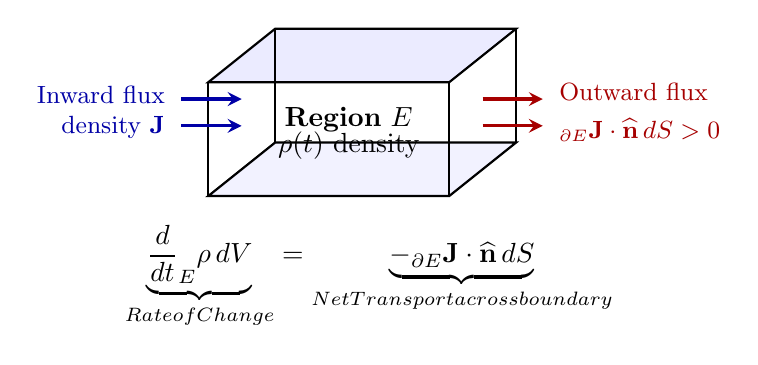
\begin{tikzpicture}[scale=0.85, >=stealth]
    % Coordinates for the box E
    \coordinate (O) at (0,0);
    \coordinate (A) at (3.6,0);
    \coordinate (B) at (4.6,0.8);
    \coordinate (C) at (1.0,0.8); % Corrected from 1.1 to 1.0
    \coordinate (D) at (0,1.7);
    \coordinate (E) at (3.6,1.7);
    \coordinate (F) at (4.6,2.5);
    \coordinate (G) at (1.0,2.5);

    % Draw the "measuring window" box
    \draw[fill=blue!5, thick] (O)--(A)--(B)--(C)--cycle;
    \draw[fill=blue!8, thick] (D)--(E)--(F)--(G)--cycle;
    \draw[thick] (O)--(D);
    \draw[thick] (A)--(E);
    \draw[thick] (B)--(F);
    \draw[thick] (C)--(G);

    % Interior state
    \node at (2.1,1.15) {\textbf{Region} \(E\)};
    \node at (2.1,0.75) {\(\rho(t)\) density};

    % Inward flux (aligned with the center of the left face)
    \draw[->, very thick, blue!65!black] (-0.4,1.45) -- ++(0.9,0);
    \draw[->, very thick, blue!65!black] (-0.4,1.05) -- ++(0.9,0);
    \node[blue!65!black, align=right, font=\small, anchor=east] at (-0.5, 1.25) {Inward flux \\ density \(\mathbf{J}\)};

    % Outward flux (aligned with the center of the right face)
    \draw[->, very thick, red!65!black] (4.1,1.45) -- ++(0.9,0);
    \draw[->, very thick, red!65!black] (4.1,1.05) -- ++(0.9,0);
    
    % Text safely spaced away from the arrow tips
    \node[red!65!black, font=\small, anchor=west, align=left] at (5.1,1.25) {Outward flux\\[1mm] \(\displaystyle \iint_{\partial E} \mathbf{J} \cdot \widehat{\mathbf{n}} \, dS > 0\)};

    % The fundamental balance equation
    \node at (2.4,-1.2)
        {\(\displaystyle \underbrace{\frac{d}{dt}\iiint_E\rho\,dV}_{\text{Rate of Change}}
        = \underbrace{-\iint_{\partial E}\mathbf J\cdot\widehat{\mathbf n}\,dS}_{\text{Net Transport across boundary}}\)};
\end{tikzpicture}
\caption{The Balance Law: For a fixed region $E$, the rate at which the stored quantity decreases is exactly equal to the net outward flux through the boundary $\partial E$. The negative sign accounts for the fact that a positive outward flux results in a loss of internal density.}
\end{figure}

\subsection{Stored amount and flux density}

The example contains the main objects.

The density
\[
    \rho
\]
measures how much material is stored per unit volume.

The flux density
\[
    \mathbf J
\]
measures how much material is transported through a unit area per unit time.

If the material has density \(\rho\) and moves with velocity
\[
    \mathbf v,
\]
then the flux density is
\[
\boxed{
    \mathbf J=\rho\mathbf v.
}
\]
A fast flow in a nearly empty region may carry little material.  A slow flow in a dense
region may carry a lot.  The product \(\rho\mathbf v\) measures what is actually being
transported.

For a fixed solid region \(E\), the stored amount is
\[
\boxed{
    \iiint_E \rho\,dV.
}
\]
The outward flux through the boundary is
\[
\boxed{
    \iint_{\partial E}\mathbf J\cdot\widehat{\mathbf n}\,dS.
}
\]

\begin{definition}[Flux density]
A \emph{flux density} is a vector field
\[
    \mathbf J
\]
whose normal component
\[
    \mathbf J\cdot\widehat{\mathbf n}
\]
measures the amount crossing a unit area per unit time in the normal direction.
\end{definition}

The sign convention is important:
\[
\begin{array}{c|c}
\mathbf J\cdot\widehat{\mathbf n}>0 & \text{net flow outward}\\[1mm]
\mathbf J\cdot\widehat{\mathbf n}<0 & \text{net flow inward}\\[1mm]
\mathbf J\cdot\widehat{\mathbf n}=0 & \text{no crossing through that surface}
\end{array}
\]

A vector tangent to the boundary may be large, but it contributes no flux across the
boundary.  It slides along the boundary instead of crossing it.

\subsection{The flux form}

The same flux can be written in the language of forms.

For a vector field
\[
    \mathbf J=(J_1,J_2,J_3),
\]
the corresponding flux \(2\)-form is
\[
\boxed{
    \Phi_{\mathbf J}
    =
    J_1\,dy\wedge dz
    +
    J_2\,dz\wedge dx
    +
    J_3\,dx\wedge dy.
}
\]
Then
\[
\boxed{
    \int_{\partial E}\Phi_{\mathbf J}
    =
    \iint_{\partial E}\mathbf J\cdot\widehat{\mathbf n}\,dS.
}
\]

For the previous example,
\[
    \mathbf J=(x,0,0),
\]
so
\[
    \Phi_{\mathbf J}=x\,dy\wedge dz.
\]
On the right face \(x=3\), this becomes
\[
    3\,dy\wedge dz.
\]
The face has \(y,z\)-area \(1\), so its contribution is \(3\).  On the left face \(x=0\),
the form is zero.  The form gives the same outward flux.

This is why flux forms were worth building.  They remember which oriented area pieces
a vector field crosses.

In the plane, the matching formula is simpler.  If
\[
    \mathbf J=(M,N),
\]
then the outward flux form on a positively oriented boundary is
\[
\boxed{
    \phi_{\mathbf J}=M\,dy-N\,dx.
}
\]
Indeed,
\[
    \int_{\partial R}\phi_{\mathbf J}
    =
    \int_{\partial R}\mathbf J\cdot\widehat{\mathbf n}\,ds.
\]
The small vector
\[
    (dy,-dx)
\]
is the outward normal times arclength when \(\partial R\) is walked with the region on
the left.

\subsection{Sources and sinks}

Some quantities are not conserved by transport alone.  Ink may be injected into water.
Heat may be produced by a heater.  Charge may be created in one model only because a
chemical reaction is supplying it.

Let
\[
    s(x,y,z,t)
\]
be the source rate per unit volume.  Positive \(s\) means creation.  Negative \(s\) means
destruction.

For a fixed solid \(E\), the total source inside \(E\) is
\[
    \iiint_E s\,dV.
\]
The full balance law becomes
\[
\boxed{
    \frac{d}{dt}\iiint_E \rho\,dV
    =
    -\iint_{\partial E}\mathbf J\cdot\widehat{\mathbf n}\,dS
    +
    \iiint_E s\,dV.
}
\]

Equivalently,
\[
\boxed{
    \frac{d}{dt}\iiint_E \rho\,dV
    +
    \iint_{\partial E}\mathbf J\cdot\widehat{\mathbf n}\,dS
    =
    \iiint_E s\,dV.
}
\]

The left side says:
\[
    \text{accumulation inside}+\text{outflow through boundary}.
\]
The right side says:
\[
    \text{creation inside}.
\]

\begin{definition}[Integral balance law]
Let \(E\) be a fixed solid region.  A density \(\rho\), flux density \(\mathbf J\), and
source rate \(s\) satisfy the integral balance law on \(E\) if
\[
\boxed{
    \frac{d}{dt}\iiint_E \rho\,dV
    +
    \iint_{\partial E}\mathbf J\cdot\widehat{\mathbf n}\,dS
    =
    \iiint_E s\,dV.
}
\]
When
\[
    s=0,
\]
the quantity is locally conserved by transport alone.
\end{definition}

In form language, the same law is
\[
\boxed{
    \frac{d}{dt}\int_E \rho\,dx\wedge dy\wedge dz
    +
    \int_{\partial E}\Phi_{\mathbf J}
    =
    \int_E s\,dx\wedge dy\wedge dz.
}
\]

\begin{example}[A source in still water]
Suppose the water is still, so
\[
    \mathbf J=\mathbf 0.
\]
Let
\[
    s(x,y,z,t)=2
\]
inside a box \(E\) of volume \(5\).  Then the balance law says
\[
    \frac{d}{dt}\iiint_E \rho\,dV
    =
    \iiint_E 2\,dV
    =
    10.
\]
The amount inside increases at rate \(10\).  Nothing crossed the boundary.  The
increase came from a source inside.
\end{example}

\subsection{What the fixed-region assumption means}

The region \(E\) in the balance law is fixed in space.  It is a window, not a moving
blob of material.

This matters.

Suppose a cloud of dye moves to the right with constant velocity.  If we follow the dye
cloud itself, the total dye in that moving blob may stay constant.  But a fixed window
on the table may first gain dye, then lose dye, as the cloud passes through.

So the balance law above is a statement for fixed control regions:
\[
    \text{watch this place, and count what enters, leaves, or is created there.}
\]

That is exactly the viewpoint needed for the divergence theorem.  The boundary
\(\partial E\) is fixed, so flux through it is well-defined.  Moving regions require an
extra transport correction.  That correction is important in fluid mechanics, but it is
not needed for the first form of conservation laws.

The balance law is still global.  It speaks about a whole region \(E\).  But if the same
balance holds for every small box we could draw inside space, then the law should have
a pointwise version.  The next step is to shrink the bookkeeping until only one local
equation remains.

\section{The continuity equation}
\label{sec:19.2}

Section \ref{sec:19.1} gave the integral balance law:
\[
    \frac{d}{dt}\iiint_E \rho\,dV
    +
    \iint_{\partial E}\mathbf J\cdot\widehat{\mathbf n}\,dS
    =
    \iiint_E s\,dV.
\]
This equation counts a whole region.  To turn it into a differential equation, we use
the divergence theorem to move the boundary flux into the interior.

\subsection{From a box balance to a local equation}

Return to the box
\[
    E=[0,3]\times[0,1]\times[0,1]
\]
from Section \ref{sec:19.1}.  There we used
\[
    \rho(x,y,z,t)=10-t,
    \qquad
    \mathbf J(x,y,z,t)=(x,0,0).
\]
There was no source:
\[
    s=0.
\]

Compute the two local terms:
\[
    \rho_t=-1,
\]
and
\[
    \nabla\cdot\mathbf J
    =
    \frac{\partial x}{\partial x}
    +
    \frac{\partial 0}{\partial y}
    +
    \frac{\partial 0}{\partial z}
    =
    1.
\]
So
\[
\boxed{
    \rho_t+\nabla\cdot\mathbf J=0.
}
\]

The global balance
\[
    A'(t)=-3
\]
was not a coincidence.  Inside every tiny box, the density decreases at rate \(1\), while
the outward spreading of the flux contributes divergence \(1\).  The two effects balance
locally.

This suggests the general local law:
\[
\boxed{
    \rho_t+\nabla\cdot\mathbf J=s.
}
\]
When there is no source,
\[
\boxed{
    \rho_t+\nabla\cdot\mathbf J=0.
}
\]
\begin{figure}[h]
\centering
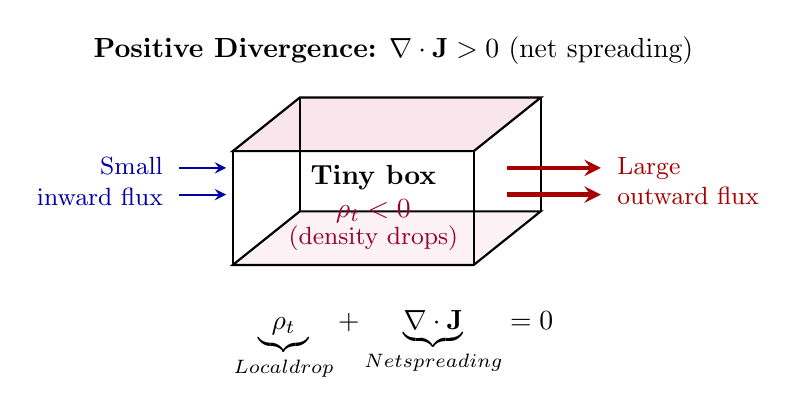
\begin{tikzpicture}[scale=0.85, >=stealth]
    % Coordinates for the differential box
    \coordinate (O) at (0,0);
    \coordinate (A) at (3.6,0);
    \coordinate (B) at (4.6,0.8);
    \coordinate (C) at (1.0,0.8);
    \coordinate (D) at (0,1.7);
    \coordinate (E) at (3.6,1.7);
    \coordinate (F) at (4.6,2.5);
    \coordinate (G) at (1.0,2.5);

    % Draw the "differential" box (shifted to purple to imply a tiny local volume)
    \draw[fill=purple!5, thick] (O)--(A)--(B)--(C)--cycle;
    \draw[fill=purple!10, thick] (D)--(E)--(F)--(G)--cycle;
    \draw[thick] (O)--(D);
    \draw[thick] (A)--(E);
    \draw[thick] (B)--(F);
    \draw[thick] (C)--(G);

    % Interior state showing a local drop in density
    \node at (2.1,1.3) {\textbf{Tiny box}};
    \node[purple!80!black] at (2.1,0.8) {\(\rho_t < 0\)};
    \node[purple!80!black, font=\small] at (2.1,0.4) {(density drops)};

    % Small inward flux (left face)
    \draw[->, thick, blue!65!black] (-0.8,1.45) -- ++(0.7,0);
    \draw[->, thick, blue!65!black] (-0.8,1.05) -- ++(0.7,0);
    \node[blue!65!black, align=right, font=\small, anchor=east] at (-0.9, 1.25) {Small \\ inward flux};

    % Large outward flux (right face)
    \draw[->, ultra thick, red!65!black] (4.1,1.45) -- ++(1.4,0);
    \draw[->, ultra thick, red!65!black] (4.1,1.05) -- ++(1.4,0);
    \node[red!65!black, font=\small, anchor=west, align=left] at (5.6,1.25) {Large \\ outward flux};

    % Divergence explanation above the box
    \node at (2.4, 3.2) {\textbf{Positive Divergence:} \(\nabla \cdot \mathbf{J} > 0\) (net spreading)};

    % The local continuity equation
    \node at (2.4,-1.2)
        {\(\displaystyle \underbrace{\rho_t}_{\text{Local drop}}
        + \underbrace{\nabla \cdot \mathbf{J}}_{\text{Net spreading}} = 0\)};
\end{tikzpicture}
\caption{The local continuity equation. If more material leaves a tiny neighborhood than enters it (\(\nabla \cdot \mathbf{J} > 0\)), the local density must drop (\(\rho_t < 0\)) to balance the loss.}
\end{figure}
\subsection{Deriving the local balance law}

Assume \(E\) is fixed.  Then, as in single-variable calculus with a parameter, the time
derivative can pass inside the integral:
\[
    \frac{d}{dt}\iiint_E \rho\,dV
    =
    \iiint_E \rho_t\,dV.
\]
The divergence theorem gives
\[
    \iint_{\partial E}\mathbf J\cdot\widehat{\mathbf n}\,dS
    =
    \iiint_E \nabla\cdot\mathbf J\,dV.
\]
Substitute both into the integral balance law:
\[
    \iiint_E \rho_t\,dV
    +
    \iiint_E \nabla\cdot\mathbf J\,dV
    =
    \iiint_E s\,dV.
\]
Combine the integrals:
\[
\boxed{
    \iiint_E
    \left(
        \rho_t+\nabla\cdot\mathbf J-s
    \right)
    dV
    =
    0.
}
\]

If this holds for every small solid region \(E\), and the integrand is continuous, then
the integrand must be zero everywhere:
\[
\boxed{
    \rho_t+\nabla\cdot\mathbf J-s=0.
}
\]
Thus
\[
\boxed{
    \rho_t+\nabla\cdot\mathbf J=s.
}
\]

\begin{theorem}[Local balance law]
Let \(\rho\), \(\mathbf J\), and \(s\) be sufficiently smooth fields on a region of space,
and suppose that the integral balance law
\[
    \frac{d}{dt}\iiint_E \rho\,dV
    +
    \iint_{\partial E}\mathbf J\cdot\widehat{\mathbf n}\,dS
    =
    \iiint_E s\,dV
\]
holds for every fixed solid region \(E\) inside that space.  Then
\[
\boxed{
    \rho_t+\nabla\cdot\mathbf J=s.
}
\]
If \(s=0\), then
\[
\boxed{
    \rho_t+\nabla\cdot\mathbf J=0.
}
\]
\end{theorem}

\begin{proof}
The proof is the calculation above, with one final observation.

Let
\[
    g=\rho_t+\nabla\cdot\mathbf J-s.
\]
The integral balance law and the divergence theorem imply
\[
    \iiint_E g\,dV=0
\]
for every fixed solid region \(E\).

If \(g(\mathbf p)>0\) at some point \(\mathbf p\), then by continuity \(g\) is still
positive in a small box around \(\mathbf p\).  The integral over that box would be
positive, not zero.  Similarly, \(g(\mathbf p)<0\) would give a small box with negative
integral.

So \(g\) must be zero at every point:
\[
    \rho_t+\nabla\cdot\mathbf J-s=0.
\]
\end{proof}

\subsection{Why the hypotheses matter}

Two small warnings prevent a common mistake.

First, an integral over one region being zero does not force the integrand to be zero.

For example,
\[
    \int_{-1}^{1} x\,dx=0,
\]
but
\[
    x
\]
is certainly not the zero function.  The positive and negative parts cancel.  That is why
the theorem needs the balance law to hold for every small region, not merely for one
large symmetric region.

Second, continuity matters if we want a pointwise equation.  Define
\[
    g(x,y,z)=
    \begin{cases}
    1, & (x,y,z)=(0,0,0),\\
    0, & \text{otherwise}.
    \end{cases}
\]
Then the ordinary triple integral of \(g\) over any solid region is \(0\), but
\[
    g(0,0,0)=1.
\]
A single point is invisible to volume integration.

Continuity rules out this kind of hidden spike.  In more advanced courses, weak or
distributional versions of conservation laws handle discontinuities such as shocks.  In
this book, the smooth case is the right first model.

\subsection{The continuity equation for moving material}

For a conserved quantity with no source,
\[
    s=0,
\]
the local law is
\[
\boxed{
    \rho_t+\nabla\cdot\mathbf J=0.
}
\]
If the material moves with velocity field
\[
    \mathbf v,
\]
then
\[
    \mathbf J=\rho\mathbf v.
\]
So the conservation law becomes
\[
\boxed{
    \rho_t+\nabla\cdot(\rho\mathbf v)=0.
}
\]

This is called the \emph{continuity equation}.

\begin{definition}[Continuity equation]
Let \(\rho(x,y,z,t)\) be a density transported by a velocity field
\[
    \mathbf v(x,y,z,t).
\]
If the quantity is conserved and has no sources or sinks, then
\[
\boxed{
    \rho_t+\nabla\cdot(\rho\mathbf v)=0.
}
\]
In coordinates, if
\[
    \mathbf v=(v_1,v_2,v_3),
\]
then
\[
\boxed{
    \rho_t+(\rho v_1)_x+(\rho v_2)_y+(\rho v_3)_z=0.
}
\]
\end{definition}

In the plane, the same equation is
\[
\boxed{
    \rho_t+(\rho v_1)_x+(\rho v_2)_y=0.
}
\]

The equation says:

\[
\boxed{
    \text{time change of density}
    +
    \text{outflow per unit volume}
    =
    0.
}
\]

\subsection{A density profile moving down a pipe}

In a long narrow pipe, suppose the velocity is constant:
\[
    v=2.
\]
The continuity equation in one spatial dimension becomes
\[
    \rho_t+(\rho v)_x=0,
\]
so
\[
    \rho_t+(2\rho)_x=0.
\]
Since \(2\) is constant,
\[
\boxed{
    \rho_t+2\rho_x=0.
}
\]

Let \(f\) be any differentiable one-variable function, and define
\[
    \rho(x,t)=f(x-2t).
\]
Then
\[
    \rho_t=-2f'(x-2t),
\]
and
\[
    \rho_x=f'(x-2t).
\]
Therefore
\[
    \rho_t+2\rho_x
    =
    -2f'(x-2t)+2f'(x-2t)
    =
    0.
\]

So every density profile of the form
\[
    f(x-2t)
\]
solves the equation.  The shape moves to the right at speed \(2\), without changing.

\begin{figure}[h]
\centering
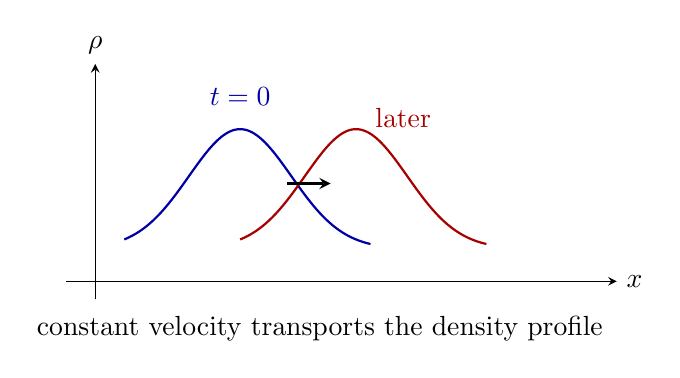
\begin{tikzpicture}[scale=0.92, >=stealth]
    \draw[->] (-0.4,0) -- (7.2,0) node[right] {\(x\)};
    \draw[->] (0,-0.25) -- (0,3.0) node[above] {\(\rho\)};

    \draw[thick, blue!65!black, domain=0.4:3.8, samples=120, smooth]
        plot (\x,{0.45+1.65*exp(-(\x-2)^2)});
    \node[blue!65!black] at (2.0,2.55) {\(t=0\)};

    \draw[thick, red!65!black, domain=2.0:5.4, samples=120, smooth]
        plot (\x,{0.45+1.65*exp(-(\x-3.6)^2)});
    \node[red!65!black] at (4.25,2.25) {later};

    \draw[->, thick] (2.65,1.35) -- (3.25,1.35);
    \node at (3.1,-0.65) {constant velocity transports the density profile};
\end{tikzpicture}
\caption{The solution \(\rho(x,t)=f(x-2t)\) moves to the right with speed \(2\).}
\end{figure}

A fixed sensor at one \(x\)-value may see the density rise and fall as the profile passes.
But a tiny observer moving with speed \(2\) sees the same density value stay with it.

\subsection{Expansion, compression, and the material derivative}

The compact equation
\[
    \rho_t+\nabla\cdot(\rho\mathbf v)=0
\]
has another useful form.  Expand the divergence using the product rule:
\[
    \nabla\cdot(\rho\mathbf v)
    =
    \mathbf v\cdot\nabla\rho
    +
    \rho\,\nabla\cdot\mathbf v.
\]
Thus
\[
\boxed{
    \rho_t+\mathbf v\cdot\nabla\rho+\rho\,\nabla\cdot\mathbf v=0.
}
\]

The first two terms are grouped together:
\[
\boxed{
    \frac{D\rho}{Dt}
    =
    \rho_t+\mathbf v\cdot\nabla\rho.
}
\]
This is the \emph{material derivative}.  It measures how \(\rho\) changes for an observer
moving with the flow.

So the continuity equation can be written as
\[
\boxed{
    \frac{D\rho}{Dt}+\rho\,\nabla\cdot\mathbf v=0.
}
\]

This separates two effects:
\[
\begin{array}{c|l}
\text{Term} & \text{Meaning} \\ \hline
\dfrac{D\rho}{Dt} & \text{density change seen by a moving particle}\\[3mm]
\rho\,\nabla\cdot\mathbf v & \text{density change forced by expansion or compression}
\end{array}
\]

\begin{example}[Expansion lowers a uniform density]
In the plane, take
\[
    \mathbf v(x,y)=(x,y).
\]
This field pushes points away from the origin.  Its divergence is
\[
    \nabla\cdot\mathbf v=1+1=2.
\]

Suppose the density is uniform in space:
\[
    \rho(x,y,t)=a(t).
\]
Then
\[
    \nabla\rho=\mathbf 0,
\]
and the continuity equation becomes
\[
    a'(t)+2a(t)=0.
\]
Hence
\[
\boxed{
    a(t)=Ce^{-2t}.
}
\]
The material is conserved, but the flow expands area, so the density decreases.
\end{example}

\begin{example}[Compression raises a uniform density]
Now take
\[
    \mathbf v(x,y)=(-x,-y).
\]
Then
\[
    \nabla\cdot\mathbf v=-1-1=-2.
\]
For a spatially uniform density
\[
    \rho(x,y,t)=a(t),
\]
the continuity equation gives
\[
    a'(t)-2a(t)=0.
\]
Therefore
\[
\boxed{
    a(t)=Ce^{2t}.
}
\]
The flow compresses material toward the origin, so density rises.
\end{example}

Divergence is not just a symbolic derivative.  It measures local expansion or
compression of the flow.

\subsection{Incompressible flow and divergence-free fields}

A flow is called \emph{incompressible} when tiny moving blobs keep the same volume
in space, or the same area in the plane.

For a smooth velocity field, incompressibility is expressed by
\[
\boxed{
    \nabla\cdot\mathbf v=0.
}
\]
A vector field with zero divergence is called \emph{divergence-free}.

If
\[
    \nabla\cdot\mathbf v=0,
\]
then the continuity equation becomes
\[
\boxed{
    \rho_t+\mathbf v\cdot\nabla\rho=0.
}
\]
Equivalently,
\[
\boxed{
    \frac{D\rho}{Dt}=0.
}
\]
The density is constant along the path of each moving particle.

\begin{example}[A rotating incompressible flow]
The swirling velocity field
\[
    \mathbf v(x,y)=(-y,x)
\]
has divergence
\[
    \nabla\cdot\mathbf v
    =
    \frac{\partial(-y)}{\partial x}
    +
    \frac{\partial x}{\partial y}
    =
    0+0
    =
    0.
\]
So the flow is incompressible.

A small blob rotates around the origin.  Its shape may turn, but to first order its area
does not grow or shrink.
\end{example}

\begin{example}[A shear flow with zero divergence]
Let
\[
    \mathbf v(x,y)=(y,0).
\]
Then
\[
    \nabla\cdot\mathbf v
    =
    \frac{\partial y}{\partial x}
    +
    \frac{\partial 0}{\partial y}
    =
    0.
\]
This flow is also incompressible.

Horizontal speed depends on height.  A small square is sheared into a slanted
parallelogram.  Its shape changes, but its area does not.

\begin{figure}[h]
\centering
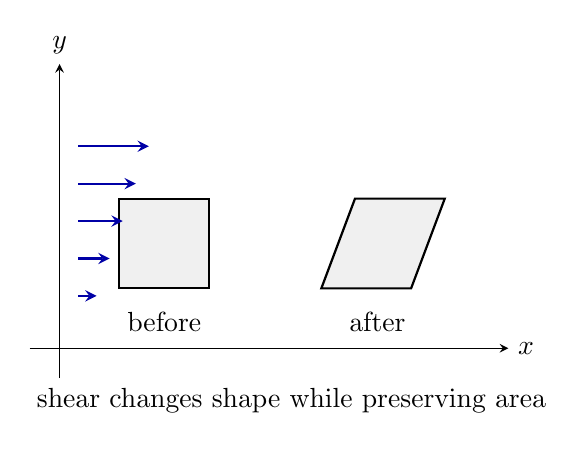
\begin{tikzpicture}[scale=0.95, >=stealth]
    \draw[->] (-0.4,0) -- (6.0,0) node[right] {\(x\)};
    \draw[->] (0,-0.4) -- (0,3.8) node[above] {\(y\)};

    \draw[fill=gray!12, thick] (0.8,0.8) rectangle (2.0,2.0);
    \node at (1.4,0.35) {before};

    \begin{scope}[shift={(2.7,0)}]
        \draw[fill=gray!12, thick]
            (0.8,0.8) -- (2.0,0.8) -- (2.45,2.0) -- (1.25,2.0) -- cycle;
        \node at (1.55,0.35) {after};
    \end{scope}

    \foreach \yy in {0.7,1.2,1.7,2.2,2.7} {
        \draw[->, blue!65!black, thick] (0.25,\yy) -- ++({0.35*\yy},0);
    }

    \node at (3.1,-0.7) {shear changes shape while preserving area};
\end{tikzpicture}
\caption{Zero divergence does not mean no motion.  It means no local area or volume
change.}
\end{figure}
\end{example}

Divergence-free motion can still rotate, shear, fold, and stir.  It simply does not create
local expansion or compression.

\subsection{The forms version of the continuity equation}

The forms language shows the structure without extra words.

In space, the stored density is the \(3\)-form
\[
    \rho\,dx\wedge dy\wedge dz.
\]
The flux density
\[
    \mathbf J=(J_1,J_2,J_3)
\]
has flux \(2\)-form
\[
    \Phi_{\mathbf J}
    =
    J_1\,dy\wedge dz
    +
    J_2\,dz\wedge dx
    +
    J_3\,dx\wedge dy.
\]
Its exterior derivative is
\[
    d\Phi_{\mathbf J}
    =
    (\nabla\cdot\mathbf J)\,dx\wedge dy\wedge dz.
\]
The local balance law
\[
    \rho_t+\nabla\cdot\mathbf J=s
\]
is therefore the form equation
\[
\boxed{
    \frac{\partial}{\partial t}
    \bigl(\rho\,dx\wedge dy\wedge dz\bigr)
    +
    d\Phi_{\mathbf J}
    =
    s\,dx\wedge dy\wedge dz.
}
\]

When \(s=0\),
\[
\boxed{
    \frac{\partial}{\partial t}
    \bigl(\rho\,dx\wedge dy\wedge dz\bigr)
    +
    d\Phi_{\mathbf J}
    =
    0.
}
\]

This is the same conservation sentence again:
\[
\boxed{
    \text{time-change of stored amount}
    +
    \text{spatial derivative of flux}
    =
    \text{source}.
}
\]

The continuity equation gives the shape of a conservation law, but it does not yet tell
us what the flux \(\mathbf J\) should be.  That choice comes from physics.  Heat flows
from hot to cold, so its flux is tied to the gradient of temperature.  Waves carry
tension and acceleration.  Equilibrium removes time and leaves a condition with no
sources.  Different stories will now begin producing equations with the same skeleton:
heat, wave, and Laplace equations.
% =====================================================================
%  Chapter 19: Conservation Laws and the Language of Fields
%  Sections 19.3 and 19.4
% =====================================================================

\section{Heat, wave, and equilibrium equations}
\label{sec:19.3}

Section \ref{sec:19.2} gave us the shape of a conservation law:
\[
    \rho_t+\nabla\cdot\mathbf J=s.
\]
The density \(\rho\) tells what is stored.  The flux \(\mathbf J\) tells what moves
across boundaries.  The source \(s\) tells what is created or destroyed inside.

That equation is not yet a physical law by itself.  It is bookkeeping.  To get a
specific equation, we must say what the flux is.  Heat, waves, and equilibrium all make
different choices, but the same few operators keep appearing:
\[
    \nabla,\qquad \nabla\cdot,\qquad \Delta.
\]

\subsection{Heat flow and the heat equation}

Imagine a thin metal plate on a table.  Let
\[
    u(x,y,t)
\]
be its temperature at the point \((x,y)\) and time \(t\).

Heat flows from warmer places toward colder places.  The gradient
\[
    \nabla u
\]
points in the direction where temperature increases fastest.  So heat should flow in the
opposite direction.

This modeling rule is called Fourier's law:
\[
\boxed{
    \mathbf J=-k\nabla u.
}
\]
Here \(k>0\) is the thermal conductivity.  A larger \(k\) means heat moves more easily
through the material.

Let
\[
    c
\]
be the heat capacity per unit area of the thin plate.  Then the stored thermal energy per
unit area is proportional to temperature:
\[
    \rho=c u.
\]
If there is no internal heat source, the conservation law says
\[
    (cu)_t+\nabla\cdot\mathbf J=0.
\]
Substitute Fourier's law:
\[
    c u_t+\nabla\cdot(-k\nabla u)=0.
\]
If \(c\) and \(k\) are constant, this becomes
\[
    c u_t-k\nabla\cdot(\nabla u)=0.
\]
The expression
\[
    \nabla\cdot(\nabla u)
\]
is the Laplacian:
\[
\boxed{
    \Delta u=u_{xx}+u_{yy}
}
\]
in the plane.  Therefore
\[
    c u_t-k\Delta u=0,
\]
or
\[
\boxed{
    u_t=\alpha\Delta u,
}
\]
where
\[
    \alpha=\frac{k}{c}
\]
is called the thermal diffusivity.

This is the heat equation.

\begin{definition}[Heat equation]
For a temperature field \(u\), the heat equation with constant diffusivity \(\alpha>0\)
is
\[
\boxed{
    u_t=\alpha\Delta u.
}
\]
In one space dimension,
\[
\boxed{
    u_t=\alpha u_{xx}.
}
\]
In two space dimensions,
\[
\boxed{
    u_t=\alpha(u_{xx}+u_{yy}).
}
\]
In three space dimensions,
\[
\boxed{
    u_t=\alpha(u_{xx}+u_{yy}+u_{zz}).
}
\]
\end{definition}

\begin{example}[A warm bump on a rod]
Consider a thin rod with coordinate \(0\le x\le1\), whose ends are held at temperature
\(0\).  Let
\[
    u(x,t)=e^{-\alpha\pi^2t}\sin(\pi x).
\]
Then
\[
    u_t=-\alpha\pi^2e^{-\alpha\pi^2t}\sin(\pi x),
\]
while
\[
    u_{xx}=-\pi^2e^{-\alpha\pi^2t}\sin(\pi x).
\]
Therefore
\[
    u_t=\alpha u_{xx}.
\]
So this is a solution of the one-dimensional heat equation.

The factor
\[
    e^{-\alpha\pi^2t}
\]
shrinks as time passes.  The sine-shaped temperature profile fades away.  Heat spreads
until the rod settles to the boundary temperature.
\end{example}

The heat equation is not just a formula.  It says that temperature changes because heat
flows down its gradient.  The Laplacian measures the net effect of that flow.

A point where
\[
    \Delta u>0
\]
is colder than its surroundings in an averaged second-order sense, so heat flows in and
\(u_t>0\).  A point where
\[
    \Delta u<0
\]
is warmer than its surroundings, so heat flows out and \(u_t<0\).

\subsection{Heat sources and nonconstant materials}

If heat is created inside the plate, the balance law is
\[
    (cu)_t+\nabla\cdot\mathbf J=s.
\]
Using
\[
    \mathbf J=-k\nabla u,
\]
we get
\[
\boxed{
    c u_t-\nabla\cdot(k\nabla u)=s.
}
\]
If \(c\) and \(k\) are constant, then
\[
\boxed{
    u_t=\alpha\Delta u+\frac{s}{c}.
}
\]

The term
\[
    \frac{s}{c}
\]
is the temperature increase forced by the source.

\begin{example}[A heater under a plate]
Suppose a small electric heater under a metal plate produces heat at rate
\[
    s(x,y,t)=10e^{-x^2-y^2}.
\]
This source is strongest near the origin and weak far away.  If the plate has constant
\(c\) and \(k\), its temperature satisfies
\[
    u_t=\alpha\Delta u+\frac{10}{c}e^{-x^2-y^2}.
\]
The first term spreads heat.  The second term creates heat.
\end{example}

The assumption
\[
    \mathbf J=-k\nabla u
\]
is a physical assumption, not a theorem of calculus.  Some materials conduct better in
one direction than another.  Then \(k\) is not just a number; it is a matrix, and the flux
law becomes
\[
    \mathbf J=-K\nabla u.
\]
The conservation law stays the same.  The constitutive law, the rule connecting flux to
the field, changes.

\subsection{Vibrating strings and the wave equation}

Heat spreads and fades.  Waves travel.

The simplest wave model is a stretched string.  Let
\[
    u(x,t)
\]
be the vertical displacement of the string at position \(x\) and time \(t\).

Take a short piece of string from \(x\) to \(x+\Delta x\).  Suppose the tension has
constant magnitude \(T\), and suppose the slopes are small.  The vertical component of
the tension at the right end is approximately
\[
    T u_x(x+\Delta x,t).
\]
The vertical component at the left end pulls the other way and is approximately
\[
    T u_x(x,t).
\]
So the net vertical force is approximately
\[
    T\bigl(u_x(x+\Delta x,t)-u_x(x,t)\bigr).
\]
For small \(\Delta x\),
\[
    u_x(x+\Delta x,t)-u_x(x,t)\approx u_{xx}(x,t)\Delta x.
\]
Thus
\[
    \text{net vertical force}\approx T u_{xx}(x,t)\Delta x.
\]

If the string has mass density \(m\) per unit length, then the mass of this small piece is
\[
    m\Delta x.
\]
Newton's law gives
\[
    m\Delta x\,u_{tt}\approx T u_{xx}\Delta x.
\]
Cancel \(\Delta x\):
\[
    m u_{tt}=T u_{xx}.
\]
Therefore
\[
\boxed{
    u_{tt}=c^2u_{xx},
}
\]
where
\[
    c^2=\frac{T}{m}.
\]

This is the one-dimensional wave equation.

\begin{definition}[Wave equation]
The wave equation in one space dimension is
\[
\boxed{
    u_{tt}=c^2u_{xx}.
}
\]
In two space dimensions, the wave equation is
\[
\boxed{
    u_{tt}=c^2\Delta u
    =
    c^2(u_{xx}+u_{yy}).
}
\]
In three space dimensions,
\[
\boxed{
    u_{tt}=c^2\Delta u
    =
    c^2(u_{xx}+u_{yy}+u_{zz}).
}
\]
\end{definition}

\begin{example}[A traveling wave]
Let
\[
    u(x,t)=f(x-ct),
\]
where \(f\) is twice differentiable.  Then
\[
    u_t=-c f'(x-ct),
\]
and
\[
    u_{tt}=c^2 f''(x-ct).
\]
Also
\[
    u_x=f'(x-ct),
\]
and
\[
    u_{xx}=f''(x-ct).
\]
Therefore
\[
    u_{tt}=c^2u_{xx}.
\]

The shape \(f\) travels to the right with speed \(c\).  Unlike heat, it does not have to
fade just because it moves.
\end{example}

There is also a left-moving wave:
\[
    u(x,t)=g(x+ct).
\]
Indeed, any sum
\[
\boxed{
    u(x,t)=f(x-ct)+g(x+ct)
}
\]
solves the one-dimensional wave equation.  This formula says that, in one dimension,
waves split naturally into right-moving and left-moving pieces.

\subsection{Vibrating membranes}

A drumhead is a two-dimensional version of the string.  Let
\[
    u(x,y,t)
\]
be its vertical displacement.  The membrane tension pulls in both the \(x\)- and
\(y\)-directions.  The net vertical force on a small rectangle is controlled by
\[
    u_{xx}+u_{yy}.
\]
Thus the model becomes
\[
\boxed{
    u_{tt}=c^2(u_{xx}+u_{yy})=c^2\Delta u.
}
\]

\begin{example}[A standing wave on a square membrane]
On the square
\[
    0\le x\le1,\qquad 0\le y\le1,
\]
consider
\[
    u(x,y,t)=\cos(\omega t)\sin(\pi x)\sin(\pi y).
\]
Then
\[
    u_{tt}=-\omega^2\cos(\omega t)\sin(\pi x)\sin(\pi y).
\]
Also
\[
    u_{xx}=-\pi^2\cos(\omega t)\sin(\pi x)\sin(\pi y),
\]
and
\[
    u_{yy}=-\pi^2\cos(\omega t)\sin(\pi x)\sin(\pi y).
\]
So
\[
    \Delta u=-2\pi^2\cos(\omega t)\sin(\pi x)\sin(\pi y).
\]
The wave equation
\[
    u_{tt}=c^2\Delta u
\]
holds exactly when
\[
    -\omega^2=-2c^2\pi^2,
\]
or
\[
\boxed{
    \omega=c\pi\sqrt2.
}
\]

This is one normal mode of the square membrane.  The shape
\[
    \sin(\pi x)\sin(\pi y)
\]
stays the same while its amplitude oscillates in time.
\end{example}

The wave equation is second order in time.  That is one visible difference between heat
and waves:
\[
\begin{array}{c|c|c}
\text{Equation} & \text{Time derivative} & \text{Behavior} \\ \hline
u_t=\alpha\Delta u & \text{first order} & \text{spreads and smooths}\\[1mm]
u_{tt}=c^2\Delta u & \text{second order} & \text{travels and oscillates}
\end{array}
\]

\subsection{Equilibrium and Laplace's equation}

Equilibrium means no time change.

For heat, equilibrium means
\[
    u_t=0.
\]
If there are no sources and the material is constant, the heat equation becomes
\[
    0=\alpha\Delta u,
\]
so
\[
\boxed{
    \Delta u=0.
}
\]

For a membrane at rest, equilibrium means
\[
    u_{tt}=0.
\]
The wave equation becomes
\[
    0=c^2\Delta u,
\]
so again
\[
\boxed{
    \Delta u=0.
}
\]

This is Laplace's equation.

\begin{definition}[Laplace's equation]
A twice differentiable function \(u\) satisfies Laplace's equation if
\[
\boxed{
    \Delta u=0.
}
\]
In the plane,
\[
\boxed{
    u_{xx}+u_{yy}=0.
}
\]
In space,
\[
\boxed{
    u_{xx}+u_{yy}+u_{zz}=0.
}
\]
A function satisfying Laplace's equation is called \emph{harmonic}.
\end{definition}

\begin{example}[A saddle that is in equilibrium]
Let
\[
    u(x,y)=x^2-y^2.
\]
Then
\[
    u_{xx}=2,
    \qquad
    u_{yy}=-2.
\]
Therefore
\[
    \Delta u=2-2=0.
\]
So \(u\) is harmonic.

Its graph is a saddle.  Equilibrium does not mean ``flat.''  It means the upward
curvature in one direction is balanced by the downward curvature in another direction.
\end{example}

\begin{example}[A steady temperature on a rectangle]
Suppose a plate has no heat sources, and its temperature is no longer changing.  Then
inside the plate
\[
    \Delta u=0.
\]
The boundary temperatures determine the solution.  If the left edge is kept hot, the
right edge cold, and the top and bottom insulated or prescribed, the interior
temperature adjusts until there is no net accumulation of heat anywhere.

The equation
\[
    \Delta u=0
\]
does not by itself tell the whole story.  Boundary conditions complete the physical
problem.
\end{example}

That last sentence is essential.  Partial differential equations almost never describe a
physical situation alone.  They need a region, boundary conditions, and often initial
conditions.

For heat, one usually needs
\[
    u(x,y,0)
\]
and boundary temperatures or boundary fluxes.

For waves, one needs both
\[
    u(x,y,0)
\]
and
\[
    u_t(x,y,0),
\]
because the equation is second order in time.

For equilibrium, there is no initial time, but the boundary data are crucial.

\subsection{Why different physical systems share the same mathematics}

The heat equation, wave equation, and Laplace equation come from different stories.

\begin{center}
\renewcommand{\arraystretch}{1.5}
\begin{tabular}{@{}l p{10cm}@{}}
    \textbf{Heat:} & thermal energy is conserved, and heat flows down the temperature gradient. \\
    \textbf{Waves:} & force equals mass times acceleration, and tension reacts to curvature. \\
    \textbf{Equilibrium:} & net flow, net force, or net source disappears.
\end{tabular}
\end{center}

Yet the same operator appears:
\(
    \Delta.
\)

The reason is geometric.  The Laplacian measures a kind of net second-order imbalance
around a point.  In one dimension, that imbalance is just
\(
    u_{xx}.
\)
In two dimensions, there are two independent coordinate directions, so the imbalance is
\[
    u_{xx}+u_{yy}.
\]
In three dimensions, it is
\[
    u_{xx}+u_{yy}+u_{zz}.
\]

A hot spot with
\[
    \Delta u<0
\]
loses heat.  A string segment with
\[
    u_{xx}<0
\]
is pulled downward.  A membrane with
\[
    \Delta u=0
\]
has its directional curvatures balanced.


The equations in this section used scalar fields: temperature, displacement, potential.
But nature also has fields that are already vectorial.  Electric fields push charges.
Magnetic fields measure flux through surfaces.  They do not merely diffuse or vibrate;
they create each other's circulation and flux.  The final capstone of the forms language
is to write those laws in the notation the book has been building from the beginning.

\section{Maxwell's equations as a forms gateway}
\label{sec:19.4}

This section is the main capstone of the book.

It is not an electromagnetism course.  We will not derive every physical constant or
solve realistic engineering problems.  The goal is different: to see why the language of
forms is not decoration.

Maxwell's equations are the place where the main ideas of the book meet:
\begin{itemize}
    \item fields attached to space,
    \item circulation along curves,
    \item flux through surfaces,
    \item sources inside volumes,
    \item the exterior derivative \(d\),
    \item the identity \(d^2=0\),
    \item and conservation laws.
\end{itemize}

Standard vector calculus treats these as four distinct formulas. The language of forms strips that away, unifying them into simple rules about boundaries and derivatives. The math doesn't obscure the physics; it reveals the underlying structure.

\subsection{Electric and magnetic fields}

Electric and magnetic fields do different kinds of measuring.

An electric field measures work per unit charge along a small displacement.  That makes
it naturally a \(1\)-form:
\[
\boxed{
    \mathcal E
    =
    E_1\,dx+E_2\,dy+E_3\,dz.
}
\]
If a unit positive charge moves by a tiny vector, \(\mathcal E\) measures the electric
work along that tiny motion.

A magnetic field is naturally measured by flux through an oriented surface.  So we write
the magnetic field as a \(2\)-form:
\[
\boxed{
    \mathcal B
    =
    B_1\,dy\wedge dz
    +
    B_2\,dz\wedge dx
    +
    B_3\,dx\wedge dy.
}
\]
This form measures magnetic flux through small oriented area pieces.

Two related fields are also useful.  The electric displacement field is a flux \(2\)-form:
\[
\boxed{
    \mathcal D
    =
    D_1\,dy\wedge dz
    +
    D_2\,dz\wedge dx
    +
    D_3\,dx\wedge dy.
}
\]
The magnetic intensity field is a circulation \(1\)-form:
\[
\boxed{
    \mathcal H
    =
    H_1\,dx+H_2\,dy+H_3\,dz.
}
\]

In vacuum, the pairs are related by physical constants:
\[
    \mathbf D=\varepsilon_0\mathbf E,
    \qquad
    \mathbf B=\mu_0\mathbf H.
\]
In materials, the relations can be more complicated.  Those relations belong to
physics.  The forms structure of Maxwell's equations does not depend on their simplest
vacuum form.

Charge density is stored in volume, so it is a \(3\)-form:
\[
\boxed{
    \mathcal Q=\rho_{\mathrm e}\,dx\wedge dy\wedge dz.
}
\]
Current density is flux of charge through surfaces, so it is a \(2\)-form:
\[
\boxed{
    \mathcal J
    =
    J_1\,dy\wedge dz
    +
    J_2\,dz\wedge dx
    +
    J_3\,dx\wedge dy.
}
\]

The roles are summarized below.

\[
\begin{array}{c|c|c}
\text{Object} & \text{Form degree} & \text{What it measures} \\ \hline
\mathcal E & 1 & \text{electric work/circulation along curves}\\[1mm]
\mathcal B & 2 & \text{magnetic flux through surfaces}\\[1mm]
\mathcal D & 2 & \text{electric flux through surfaces}\\[1mm]
\mathcal H & 1 & \text{magnetic circulation along curves}\\[1mm]
\mathcal Q & 3 & \text{charge stored in volumes}\\[1mm]
\mathcal J & 2 & \text{charge current through surfaces}
\end{array}
\]

This table is already half the story.  The degree of each form tells us what kind of
geometric object it belongs to.

\subsection{The four equations in forms language}

At each fixed time, Maxwell's equations can be written as
\[
\boxed{
    d\mathcal D=\mathcal Q,
}
\]
\[
\boxed{
    d\mathcal B=0,
}
\]
\[
\boxed{
    d\mathcal E+\frac{\partial\mathcal B}{\partial t}=0,
}
\]
and
\[
\boxed{
    d\mathcal H-\frac{\partial\mathcal D}{\partial t}=\mathcal J.
}
\]

These are Maxwell's equations in three-dimensional space, written with spatial forms.

Here is the translation into vector notation:

\[
\begin{array}{c|c|c}
\text{Name} & \text{Forms version} & \text{Vector version} \\ \hline
\text{Gauss for electricity}
& d\mathcal D=\mathcal Q
& \nabla\cdot\mathbf D=\rho_{\mathrm e}
\\[2mm]
\text{Gauss for magnetism}
& d\mathcal B=0
& \nabla\cdot\mathbf B=0
\\[2mm]
\text{Faraday's law}
& d\mathcal E+\mathcal B_t=0
& \nabla\times\mathbf E+\mathbf B_t=0
\\[2mm]
\text{Ampere--Maxwell law}
& d\mathcal H-\mathcal D_t=\mathcal J
& \nabla\times\mathbf H-\mathbf D_t=\mathbf J
\end{array}
\]

The forms equations are not shorter only because of notation.  They say which kind of
integral each law wants.

\[
\begin{array}{c|c}
\text{Equation} & \text{Natural integral form} \\ \hline
d\mathcal D=\mathcal Q
& \displaystyle \int_{\partial E}\mathcal D=\int_E\mathcal Q
\\[3mm]
d\mathcal B=0
& \displaystyle \int_{\partial E}\mathcal B=0
\\[3mm]
d\mathcal E+\mathcal B_t=0
& \displaystyle \int_{\partial S}\mathcal E
=
-\frac{d}{dt}\int_S\mathcal B
\\[3mm]
d\mathcal H-\mathcal D_t=\mathcal J
& \displaystyle \int_{\partial S}\mathcal H
=
\int_S\mathcal J+\frac{d}{dt}\int_S\mathcal D
\end{array}
\]

These integral forms are where the equations become physical.

\subsection{Gauss's law: charge is detected by electric flux}

The equation
\[
    d\mathcal D=\mathcal Q
\]
says that the exterior derivative of the electric flux form is the charge density
\(3\)-form.

Let \(E\) be a solid region.  Stokes' theorem gives
\[
    \int_{\partial E}\mathcal D
    =
    \int_E d\mathcal D
    =
    \int_E\mathcal Q.
\]
So
\[
\boxed{
    \int_{\partial E}\mathcal D
    =
    \int_E \rho_{\mathrm e}\,dV.
}
\]
In words:

\[
\boxed{
    \text{electric flux through a closed surface}
    =
    \text{charge enclosed.}
}
\]

The boundary surface detects what is stored inside.

\begin{example}[A point charge, seen from outside]
A positive point charge at the origin creates electric flux through every sphere around
it.  In a fully realistic treatment, the charge density is concentrated at a point, so it is
not an ordinary continuous function.  The smooth version of Stokes' theorem in this
book does not directly handle that singularity.

But the moral is exactly the same as the warning examples in Chapter \ref{ch:18}:
a closed surface can detect something inside.  If a field is singular at a missing point,
we cannot apply the ordinary smooth theorem across that point as though nothing were
there.
\end{example}

For smooth charge density, there is no singularity.  The law simply says that charge is
the source of electric flux.

\subsection{No magnetic monopoles: magnetic flux has no source}

The magnetic equation
\[
    d\mathcal B=0
\]
says that magnetic flux has no volume source.

Let \(E\) be a solid region.  Then
\[
    \int_{\partial E}\mathcal B
    =
    \int_E d\mathcal B
    =
    0.
\]
Thus
\[
\boxed{
    \int_{\partial E}\mathcal B=0.
}
\]

In vector language,
\[
\boxed{
    \iint_{\partial E}\mathbf B\cdot\widehat{\mathbf n}\,dS=0.
}
\]

Magnetic field lines may pass through a closed surface, but as much flux enters as
leaves.  There is no isolated magnetic charge inside the region.

\begin{example}[A uniform magnetic field through a box]
Let
\[
    \mathbf B=(0,0,B_0),
\]
so
\[
    \mathcal B=B_0\,dx\wedge dy.
\]
For a rectangular box, the top face has upward orientation and contributes positive
flux
\[
    B_0(\text{area of top}).
\]
The bottom face has downward orientation and contributes the negative of the same
amount.  The side faces contribute \(0\), because the field is tangent to them.

The total magnetic flux through the closed box is
\[
    0.
\]
\end{example}

Again the sign is not decoration.  Flux through a closed surface is an oriented sum.
Entering and leaving must be counted with opposite signs.

\subsection{Faraday's law: changing magnetic flux creates electric circulation}

Faraday's law is
\[
\boxed{
    d\mathcal E+\frac{\partial\mathcal B}{\partial t}=0.
}
\]
Let \(S\) be an oriented surface with boundary \(\partial S\).  Integrate over \(S\):
\[
    \int_S d\mathcal E
    +
    \int_S \frac{\partial\mathcal B}{\partial t}
    =
    0.
\]
By Stokes' theorem,
\[
    \int_S d\mathcal E=\int_{\partial S}\mathcal E.
\]
So
\[
\boxed{
    \int_{\partial S}\mathcal E
    =
    -\frac{d}{dt}\int_S\mathcal B.
}
\]

In words:

\[
\boxed{
    \text{electric circulation around a loop}
    =
    -\text{rate of change of magnetic flux through the loop.}
}
\]

This is one of the cleanest places to see why a \(1\)-form and a \(2\)-form belong in
the same theorem.  The electric field is integrated around a boundary curve.  The
magnetic field is integrated through a surface spanning that curve.

\begin{example}[A changing magnetic field through a circular loop]
Let \(S\) be the disk
\[
    x^2+y^2\le R^2,\qquad z=0,
\]
oriented upward.  Its boundary circle is oriented counterclockwise as viewed from
above.

Suppose the magnetic field is vertical and spatially uniform:
\[
    \mathcal B=b(t)\,dx\wedge dy.
\]
Then
\[
    \int_S\mathcal B=b(t)\pi R^2.
\]
Faraday's law gives
\[
\boxed{
    \int_{\partial S}\mathcal E
    =
    -b'(t)\pi R^2.
}
\]

If \(b'(t)>0\), then the upward magnetic flux is increasing, and the induced electric
circulation is negative relative to the counterclockwise orientation.  That means the
electric circulation is clockwise when viewed from above.

The minus sign is the mathematical form of Lenz's law: the induced circulation opposes
the change in magnetic flux.
\end{example}

We can even find one possible electric form in this symmetric example.  Recall that
\[
    d(-y\,dx+x\,dy)=2\,dx\wedge dy.
\]
If
\[
    \mathcal E=-\frac{b'(t)}{2}(-y\,dx+x\,dy),
\]
then
\[
    d\mathcal E=-b'(t)\,dx\wedge dy.
\]
Since
\[
    \mathcal B_t=b'(t)\,dx\wedge dy,
\]
we get
\[
    d\mathcal E+\mathcal B_t=0.
\]
So this \(\mathcal E\) satisfies Faraday's law.

\subsection{Ampere--Maxwell law: current and changing electric flux create magnetic circulation}

The fourth equation is
\[
\boxed{
    d\mathcal H-\frac{\partial\mathcal D}{\partial t}=\mathcal J.
}
\]
Equivalently,
\[
\boxed{
    d\mathcal H=\mathcal J+\frac{\partial\mathcal D}{\partial t}.
}
\]

Integrate over an oriented surface \(S\):
\[
    \int_S d\mathcal H
    =
    \int_S\mathcal J
    +
    \frac{d}{dt}\int_S\mathcal D.
\]
By Stokes' theorem,
\[
    \int_S d\mathcal H=\int_{\partial S}\mathcal H.
\]
Therefore
\[
\boxed{
    \int_{\partial S}\mathcal H
    =
    \int_S\mathcal J
    +
    \frac{d}{dt}\int_S\mathcal D.
}
\]

In words:

\[
\boxed{
    \text{magnetic circulation around a loop}
    =
    \text{current through the loop}
    +
    \text{changing electric flux through the loop.}
}
\]

The second term,
\[
    \frac{\partial\mathcal D}{\partial t},
\]
is Maxwell's displacement-current term.  It is not a decorative correction.  It is the
term that makes the equation compatible with conservation of charge.

\subsection{One loop, two surfaces: why Maxwell's correction is necessary}

This example is the heart of the capstone.

Picture a wire charging a parallel-plate capacitor.  A current flows through the wire
toward one plate.  Between the plates there is no conduction current crossing the gap,
but the electric field between the plates is changing.

Let \(C\) be a loop around the wire.  The loop can be spanned by many different
surfaces.

One surface, call it \(S_1\), cuts through the wire.  The current flux through \(S_1\) is
\[
    \int_{S_1}\mathcal J=I.
\]

Another surface, call it \(S_2\), bulges out between the capacitor plates and crosses the
gap instead of cutting the wire.  No conduction current crosses this surface:
\[
    \int_{S_2}\mathcal J=0.
\]

If the law were only
\[
    d\mathcal H=\mathcal J,
\]
then Stokes' theorem would give
\[
    \int_C\mathcal H=\int_{S_1}\mathcal J=I
\]
using \(S_1\), but
\[
    \int_C\mathcal H=\int_{S_2}\mathcal J=0
\]
using \(S_2\).

That is impossible.  The same boundary loop \(C\) cannot have two different magnetic
circulations.

Maxwell's corrected law says
\[
    d\mathcal H=\mathcal J+\mathcal D_t.
\]
Now the two surfaces agree.

For \(S_1\), the conduction current contributes
\[
    \int_{S_1}\mathcal J=I.
\]
For \(S_2\), the changing electric flux contributes
\[
    \frac{d}{dt}\int_{S_2}\mathcal D=I.
\]
So both surfaces give
\[
\boxed{
    \int_C\mathcal H=I.
}
\]

\begin{figure}[h]
\centering
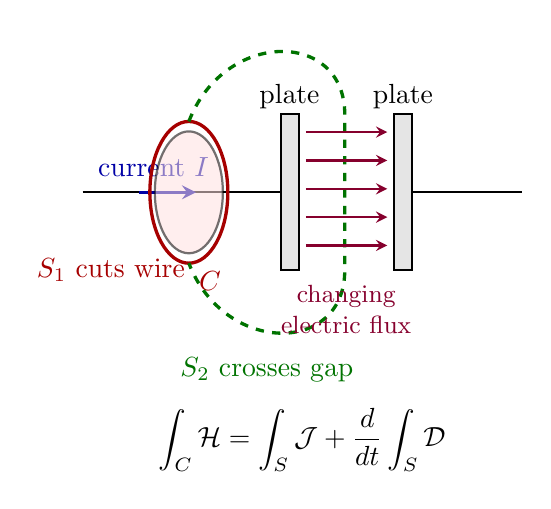
\begin{tikzpicture}[scale=0.9, >=stealth]
    % plates
    \draw[fill=gray!20, thick] (3.0,1.0) rectangle (3.25,3.2);
    \draw[fill=gray!20, thick] (4.6,1.0) rectangle (4.85,3.2);
    \node at (3.12,3.45) {plate};
    \node at (4.72,3.45) {plate};

    % wires
    \draw[thick] (0.2,2.1) -- (3.0,2.1);
    \draw[thick] (4.85,2.1) -- (6.4,2.1);

    \draw[->, very thick, blue!65!black] (1.0,2.1) -- (1.8,2.1);
    \node[blue!65!black] at (1.2,2.45) {current \(I\)};

    % loop C
    \draw[red!65!black, very thick] (1.7,2.1) ellipse (0.55 and 1.0);
    \node[red!65!black] at (2.0,0.85) {\(C\)};

    % surface S1
    \draw[fill=red!12, opacity=0.55, thick] (1.7,2.1) ellipse (0.48 and 0.86);
    \node[red!65!black] at (0.6,1.0) {\(S_1\) cuts wire};

    % surface S2 schematic (adjusted to arc wider and avoid text)
    \draw[green!45!black, very thick, dashed]
        (1.7,3.1) .. controls (2.2,4.4) and (3.9,4.4) .. (3.9,3.2)
        .. controls (3.9,2.6) and (3.9,1.6) .. (3.9,1.0)
        .. controls (3.9,-0.2) and (2.2,-0.2) .. (1.7,1.1);
    
    % label for S2 (moved below the bottom arc)
    \node[green!45!black] at (2.8,-0.4) {\(S_2\) crosses gap};

    % electric flux between plates
    \foreach \y in {1.35,1.75,2.15,2.55,2.95} {
        \draw[->, purple!70!black, thick] (3.35,\y) -- (4.5,\y);
    }
    
    % flux label (stacked and placed safely below the gap)
    \node[purple!70!black, align=center, font=\small] at (3.92,0.45) 
        {changing \\ electric flux};

    % formula (shifted further down to clear the S2 label)
    \node at (3.3,-1.4)
        {\(\displaystyle \int_C\mathcal H
        =
        \int_S\mathcal J+\frac{d}{dt}\int_S\mathcal D\)};
\end{tikzpicture}
\caption{The same loop can bound different surfaces. Maxwell's displacement-current
term makes the answer independent of the spanning surface.}
\end{figure}

This example shows the power of the forms viewpoint.  A boundary integral should not
depend on which spanning surface we use, unless something singular or omitted lies
between the surfaces.  The displacement-current term is exactly what restores that
surface independence during charging.

\subsection{Charge conservation from \texorpdfstring{\(d^2=0\)}{d squared equals zero}}

Now the continuity equation returns.

Start with Ampere--Maxwell:
\[
    d\mathcal H-\mathcal D_t=\mathcal J.
\]
Apply \(d\) to both sides:
\[
    d(d\mathcal H)-d(\mathcal D_t)=d\mathcal J.
\]
Since
\[
    d^2=0,
\]
we have
\[
    d(d\mathcal H)=0.
\]
Also, time differentiation commutes with the spatial exterior derivative:
\[
    d(\mathcal D_t)=(d\mathcal D)_t.
\]
By Gauss's law,
\[
    d\mathcal D=\mathcal Q.
\]
Therefore
\[
    -\mathcal Q_t=d\mathcal J.
\]
So
\[
\boxed{
    \mathcal Q_t+d\mathcal J=0.
}
\]

This is charge conservation.

In vector notation,
\[
\mathcal Q=\rho_{\mathrm e}\,dx\wedge dy\wedge dz,
\]
and
\[
d\mathcal J=(\nabla\cdot\mathbf J)\,dx\wedge dy\wedge dz.
\]
Thus
\[
\boxed{
    \rho_{\mathrm e,t}+\nabla\cdot\mathbf J=0.
}
\]

This is the continuity equation from Section \ref{sec:19.2}, now forced by Maxwell's
equations.

The logic is worth pausing over:

\[
\boxed{
\begin{array}{c}
\text{Ampere--Maxwell law}\\
+\ \text{Gauss's law}\\
+\ d^2=0
\end{array}
\quad\Longrightarrow\quad
\text{conservation of charge.}
}
\]

This is one of the deepest payoffs of the notation.  Conservation is not pasted onto the
equations afterward.  It is built into their differential-form structure.

\subsection{The homogeneous equations and potentials}

Two of Maxwell's equations have no source terms:
\[
    d\mathcal B=0,
\]
and
\[
    d\mathcal E+\mathcal B_t=0.
\]
They are called the homogeneous equations.

The first says that \(\mathcal B\) is closed:
\[
    d\mathcal B=0.
\]
On a simple enough region, closed forms are locally exact.  So locally we can write
\[
\boxed{
    \mathcal B=d\mathcal A
}
\]
for some \(1\)-form \(\mathcal A\), called the magnetic vector potential.

Then Faraday's law becomes
\[
    d\mathcal E+\frac{\partial}{\partial t}(d\mathcal A)=0.
\]
Because \(d\) and \(\partial/\partial t\) commute,
\[
    d(\mathcal E+\mathcal A_t)=0.
\]
Again, locally a closed \(1\)-form is exact.  So we can write
\[
    \mathcal E+\mathcal A_t=-d\varphi,
\]
or
\[
\boxed{
    \mathcal E=-d\varphi-\mathcal A_t.
}
\]
The function \(\varphi\) is the electric scalar potential.

These formulas are not needed to use Maxwell's equations, but they show another place
where the identity
\[
    d^2=0
\]
organizes the theory.

There is a warning from Chapter \ref{ch:17}: closed does not always mean globally
exact.  Missing points, holes, and topology can matter.  The equation
\[
    d\mathcal B=0
\]
is local.  Writing
\[
    \mathcal B=d\mathcal A
\]
globally may require assumptions about the region.

\subsection{What changes in space-time}

So far, time has been a parameter.  At each time \(t\), we wrote forms on ordinary
space:
\[
    \mathcal E,\quad \mathcal B,\quad \mathcal D,\quad \mathcal H.
\]

But Maxwell's equations are really space-time equations.  Time is not merely a label
outside the geometry.  It joins the coordinates:
\[
    (t,x,y,z).
\]

Let
\(
    d_4
\)
denote the exterior derivative in space-time.  It differentiates with respect to \(t\),
\(x\), \(y\), and \(z\).

With one sign convention, define the electromagnetic field \(2\)-form
\[
\boxed{
    F=\mathcal B+\mathcal E\wedge dt.
}
\]
Then
\[
\begin{aligned}
d_4F
&=
d\mathcal B
+
dt\wedge\left(\mathcal B_t+d\mathcal E\right).
\end{aligned}
\]
Therefore
\[
\boxed{
    d_4F=0
}
\]
is exactly the pair
\[
    d\mathcal B=0,
\]
\[
    d\mathcal E+\mathcal B_t=0.
\]
So the no-magnetic-monopoles law and Faraday's law combine into one space-time
equation:
\[
\boxed{
    d_4F=0.
}
\]

The other pair also combines.  Define
\[
\boxed{
    G=\mathcal D-\mathcal H\wedge dt.
}
\]
Then
\[
\begin{aligned}
d_4G
&=
d\mathcal D
+
dt\wedge(\mathcal D_t-d\mathcal H).
\end{aligned}
\]
Using
\[
    d\mathcal D=\mathcal Q
\]
and
\[
    d\mathcal H-\mathcal D_t=\mathcal J,
\]
we get
\[
\boxed{
    d_4G=\mathcal Q-dt\wedge\mathcal J.
}
\]
The right side is the space-time current \(3\)-form:
\[
\boxed{
    \mathscr J=\mathcal Q-dt\wedge\mathcal J.
}
\]
So the second pair becomes
\[
\boxed{
    d_4G=\mathscr J.
}
\]

Now apply \(d_4\) again:
\[
    d_4(d_4G)=d_4\mathscr J.
\]
Since
\[
    d_4^2=0,
\]
we get
\[
\boxed{
    d_4\mathscr J=0.
}
\]
That is charge conservation in space-time.

The space-time form of Maxwell's equations is therefore
\[
\boxed{
    d_4F=0,
}
\]
\[
\boxed{
    d_4G=\mathscr J.
}
\]

This is the gateway.

Electric and magnetic fields are no longer two unrelated vector fields.  They are pieces
of space-time forms.  The equations are no longer four separate vector identities.  They
are two exterior-derivative equations, with conservation following from
\[
    d_4^2=0.
\]

A later course explains how the geometry of space-time relates \(F\) and \(G\).  That
relationship uses the metric of space-time, and the operation that appears there is the
Hodge star.  We do not need it here.  The point for this book is simpler and more
important:

\[
\boxed{
    \text{the language of forms is the natural language of Maxwell's equations.}
}
\]

\subsection{The book's main arc, seen from the end}

The book began with a displacement:
\[
    (3,4).
\]
It was only an instruction to move.

Then we learned that vectors could measure length, area, and volume.  The wedge
product remembered orientation:
\[
    dx\wedge dy,
    \qquad
    dx\wedge dy\wedge dz.
\]
Functions became \(0\)-forms.  Work integrands became \(1\)-forms.  Flux integrands
became \(2\)-forms.  Densities became \(3\)-forms.

The exterior derivative connected them:
\[
    0\text{-forms}\xrightarrow{d}1\text{-forms}
    \xrightarrow{d}2\text{-forms}
    \xrightarrow{d}3\text{-forms}.
\]
In vector language, those arrows became
\[
    \nabla,\qquad \nabla\times,\qquad \nabla\cdot.
\]
The identity
\[
    d^2=0
\]
became the quiet reason behind
\[
    \nabla\times\nabla f=\mathbf 0
\]
and
\[
    \nabla\cdot(\nabla\times\mathbf F)=0.
\]

Stokes' theorem then said:
\[
    \int_{\partial M}\omega=\int_M d\omega.
\]
Boundary measurements and interior derivatives were two views of the same thing.

Finally, conservation laws added time.  The continuity equation said:
\[
    \text{time change of stored amount}
    +
    \text{spatial derivative of flux}
    =
    \text{source}.
\]
Heat, waves, and equilibrium showed how physical assumptions choose fluxes and forces.

Maxwell's equations show the whole structure at once.  Electric circulation, magnetic
flux, charge density, current flux, Stokes' theorem, \(d\), and \(d^2=0\) all appear in
one system.

So the final lesson is not a formula.  It is a way of seeing.

\[
\boxed{
\begin{array}{c}
\text{Local derivatives describe what happens inside.}\\[1mm]
\text{Boundary integrals record what crosses or circulates outside.}\\[1mm]
\text{Differential forms keep the dimensions and orientations honest.}
\end{array}
}
\]

That is the promise of multivariable calculus fulfilled: from tiny changes near one
point to global laws over curves, surfaces, solids, and finally space-time.
% =====================================================================
%  Chapter 19: Conservation Laws and the Language of Fields
%  Sections 19.5 and 19.6
% =====================================================================

\section{Potential theory and harmonic functions}
\label{sec:19.5}

Maxwell's equations were the broad capstone: fields, flux, circulation, sources,
boundaries, and the identity \(d^2=0\) all appeared together.  This section is a quieter
coda.  It returns to one scalar field
\[
    u(x,y,z),
\]
but now we read it with the whole book behind us.

A scalar field can be a temperature, an electric potential, a height, or a pressure.
When its gradient field has no source inside a region, the field satisfies
\[
    \Delta u=0.
\]
Those functions are called harmonic.  They are the steady states of heat flow, the
potentials of source-free fields, and the energy-minimizing shapes among all functions
with the same boundary values.

\subsection{The Laplacian as divergence of the gradient}

Start with steady heat in a thin metal plate.  Let
\[
    u(x,y)
\]
be the temperature.  Fourier's law says heat flows down the temperature gradient:
\[
    \mathbf J=-k\nabla u,
\]
where \(k>0\) is constant.

If there are no heat sources inside the plate and the temperature is no longer changing,
then the local balance law from Section \ref{sec:19.2} becomes
\[
    \nabla\cdot\mathbf J=0.
\]
Substitute the flux law:
\[
    \nabla\cdot(-k\nabla u)=0.
\]
Since \(k\) is constant,
\[
    -k\nabla\cdot(\nabla u)=0.
\]
So
\[
\boxed{
    \nabla\cdot(\nabla u)=0.
}
\]

This expression is the Laplacian:
\[
\boxed{
    \Delta u=\nabla\cdot(\nabla u).
}
\]

In coordinates,
\[
\boxed{
    \Delta u=u_{xx}+u_{yy}
}
\]
in the plane, and
\[
\boxed{
    \Delta u=u_{xx}+u_{yy}+u_{zz}
}
\]
in space.

\begin{definition}[Laplacian]
For a twice differentiable scalar field \(u\), the \emph{Laplacian} of \(u\) is
\[
\boxed{
    \Delta u=\nabla\cdot(\nabla u).
}
\]
In \(\mathbb R^2\),
\[
    \Delta u=u_{xx}+u_{yy}.
\]
In \(\mathbb R^3\),
\[
    \Delta u=u_{xx}+u_{yy}+u_{zz}.
\]
\end{definition}

\begin{example}[A source-free temperature pattern]
Let
\[
    u(x,y)=e^x\cos y.
\]
Then
\[
    u_{xx}=e^x\cos y,
\]
while
\[
    u_{yy}=-e^x\cos y.
\]
Therefore
\[
    \Delta u=u_{xx}+u_{yy}=0.
\]
This field can describe a steady temperature pattern with no internal heat sources,
provided the boundary temperatures are chosen to match it.
\end{example}

There is also a forms version.  In the plane, the flux form of the gradient field
\[
    \nabla u=(u_x,u_y)
\]
is
\[
\boxed{
    \phi_{\nabla u}=u_x\,dy-u_y\,dx.
}
\]
Then
\[
\begin{aligned}
d\phi_{\nabla u}
&=
d(u_x\,dy-u_y\,dx)\\
&=
u_{xx}\,dx\wedge dy-u_{yy}\,dy\wedge dx\\
&=
(u_{xx}+u_{yy})\,dx\wedge dy\\
&=
\Delta u\,dx\wedge dy.
\end{aligned}
\]
So
\[
\boxed{
    d\phi_{\nabla u}=\Delta u\,dx\wedge dy.
}
\]

In space, the flux form of \(\nabla u\) is
\[
\boxed{
    \Phi_{\nabla u}
    =
    u_x\,dy\wedge dz
    +
    u_y\,dz\wedge dx
    +
    u_z\,dx\wedge dy.
}
\]
Its exterior derivative is
\[
\boxed{
    d\Phi_{\nabla u}
    =
    \Delta u\,dx\wedge dy\wedge dz.
}
\]

So the Laplacian is the coefficient of the exterior derivative of the gradient flux form.
It measures the source strength of the gradient field.

\subsection{Harmonic functions}

A function with zero Laplacian gets its own name.

\begin{definition}[Harmonic function]
A twice differentiable function \(u\) is called \emph{harmonic} on a region \(D\) if
\[
\boxed{
    \Delta u=0
}
\]
at every point of \(D\).
\end{definition}

A harmonic function has a gradient field with no source inside the region:
\[
    \nabla\cdot(\nabla u)=0.
\]
Equivalently,
\[
    d\Phi_{\nabla u}=0
\]
in space, or
\[
    d\phi_{\nabla u}=0
\]
in the plane.

\begin{example}[A saddle in balance]
Let
\[
    u(x,y)=x^2-y^2.
\]
Then
\[
    u_{xx}=2,
    \qquad
    u_{yy}=-2.
\]
So
\[
    \Delta u=2-2=0.
\]
The graph is a saddle.  Harmonic does not mean flat.  It means that the upward bending
in one direction balances the downward bending in another.
\end{example}

\begin{theorem}[Harmonic functions have zero gradient flux through small boundaries]
Let \(u\) be \(C^2\) on a region \(D\).  Then \(u\) is harmonic on \(D\) if and only if,
for every small solid region \(E\subset D\),
\[
\boxed{
    \int_{\partial E}\Phi_{\nabla u}=0.
}
\]
In the plane, the corresponding statement is
\[
\boxed{
    \int_{\partial R}\phi_{\nabla u}=0
}
\]
for every small plane region \(R\subset D\).
\end{theorem}

\begin{proof}
In space, Stokes' theorem gives
\[
    \int_{\partial E}\Phi_{\nabla u}
    =
    \int_E d\Phi_{\nabla u}
    =
    \int_E \Delta u\,dx\wedge dy\wedge dz.
\]
If \(\Delta u=0\), every such boundary flux is \(0\).

Conversely, if the boundary flux is \(0\) for every small \(E\), then
\[
    \int_E \Delta u\,dV=0
\]
for every small \(E\).  Since \(\Delta u\) is continuous, the same argument used in
Section \ref{sec:19.2} forces
\[
    \Delta u=0
\]
pointwise.

The plane proof is the same, with \(dA\) replacing \(dV\).
\end{proof}

The hypotheses matter.  The function must be defined and smooth on the whole region
where we apply the theorem.

\begin{example}[A hidden source at a missing point]
On the punctured plane
\[
    \mathbb R^2\setminus\{(0,0)\},
\]
define
\[
    u(x,y)=\log r,
    \qquad
    r=\sqrt{x^2+y^2}.
\]
Away from the origin, \(u\) is harmonic:
\[
    \Delta u=0.
\]
But its gradient is
\[
    \nabla u=\left(\frac{x}{r^2},\frac{y}{r^2}\right).
\]

On the circle \(r=a\), the outward unit normal is
\[
    \widehat{\mathbf n}=\left(\frac{x}{a},\frac{y}{a}\right),
\]
and
\[
    \nabla u\cdot\widehat{\mathbf n}
    =
    \frac{1}{a}.
\]
Since \(ds=a\,d\theta\),
\[
\begin{aligned}
    \int_{r=a}\nabla u\cdot\widehat{\mathbf n}\,ds
    &=
    \int_0^{2\pi}\frac1a(a\,d\theta)\\
    &=
    2\pi.
\end{aligned}
\]

This does not contradict the theorem.  The disk \(r\le a\) contains the origin, where
\(\log r\) is not defined.  The missing point behaves like a hidden source.  A theorem
about smooth functions on a whole region cannot be applied across a hole in the
domain.
\end{example}

This example is the same kind of warning we saw for closed but non-exact forms.  A
puncture in the region can carry information that no local derivative sees away from
the puncture.

\subsection{Mean value ideas}

Harmonic functions have a surprising averaging property: the value at the center of a
circle is the average value on the circle.

First see it in a concrete example.  Let
\[
    u(x,y)=x^2-y^2.
\]
Take a circle of radius \(r\) centered at \((a,b)\):
\[
    x=a+r\cos\theta,
    \qquad
    y=b+r\sin\theta.
\]
Then
\[
\begin{aligned}
u(a+r\cos\theta,b+r\sin\theta)
&=
(a+r\cos\theta)^2-(b+r\sin\theta)^2\\
&=
a^2-b^2
+2ar\cos\theta
-2br\sin\theta\\
&\qquad
+r^2(\cos^2\theta-\sin^2\theta).
\end{aligned}
\]
Average from \(0\) to \(2\pi\).  The average of \(\cos\theta\) is \(0\), the average of
\(\sin\theta\) is \(0\), and the average of
\[
    \cos^2\theta-\sin^2\theta=\cos(2\theta)
\]
is also \(0\).  So the circular average is
\[
    a^2-b^2.
\]
But
\[
    u(a,b)=a^2-b^2.
\]
Thus
\[
\boxed{
    \text{average of }u\text{ on the circle}=u\text{ at the center.}
}
\]

\begin{figure}[h]
\centering
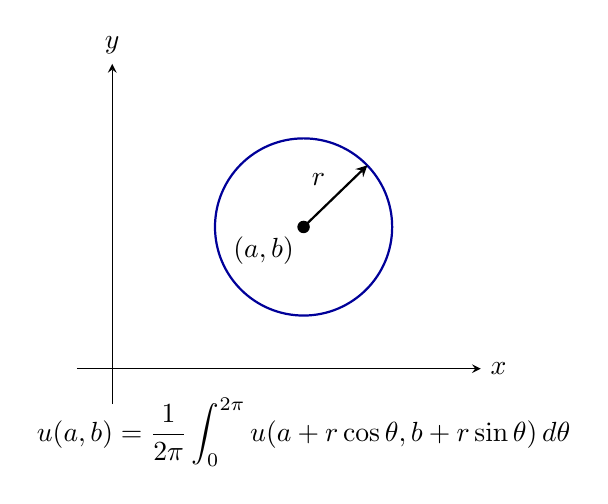
\begin{tikzpicture}[scale=0.9, >=stealth]
    \draw[->] (-0.5,0) -- (5.2,0) node[right] {\(x\)};
    \draw[->] (0,-0.5) -- (0,4.3) node[above] {\(y\)};

    \coordinate (C) at (2.7,2.0);
    \draw[thick, blue!60!black] (C) circle (1.25);

    \fill (C) circle (2.5pt);
    \node[below left] at (C) {\((a,b)\)};

    \draw[->, thick] (C) -- ++(0.9,0.87)
        node[midway, above left] {\(r\)};

    \node at (2.7,-0.9)
        {\(\displaystyle u(a,b)=\frac1{2\pi}\int_0^{2\pi}
        u(a+r\cos\theta,b+r\sin\theta)\,d\theta\)};
\end{tikzpicture}
\caption{A harmonic function is balanced: its center value equals its circular average.}
\end{figure}

The example is not a coincidence.

\begin{theorem}[Mean value property]
Let \(u\) be harmonic on a disk containing the closed disk
\[
    (x-a)^2+(y-b)^2\le r^2.
\]
Then
\[
\boxed{
    u(a,b)
    =
    \frac1{2\pi}\int_0^{2\pi}
    u(a+r\cos\theta,b+r\sin\theta)\,d\theta.
}
\]
That is, the value at the center equals the average value on every circle around it,
as long as the whole closed disk lies inside the domain.
\end{theorem}

\begin{proof}
Let
\[
    A(r)=\frac1{2\pi}\int_0^{2\pi}
    u(a+r\cos\theta,b+r\sin\theta)\,d\theta.
\]
Differentiate with respect to \(r\):
\[
    A'(r)
    =
    \frac1{2\pi}\int_0^{2\pi}
    \nabla u\cdot(\cos\theta,\sin\theta)\,d\theta.
\]
On the circle of radius \(r\), the outward unit normal is
\[
    \widehat{\mathbf n}=(\cos\theta,\sin\theta),
\]
and
\[
    ds=r\,d\theta.
\]
So
\[
    A'(r)
    =
    \frac1{2\pi r}
    \int_{C_r}\nabla u\cdot\widehat{\mathbf n}\,ds.
\]
By the divergence theorem in the plane,
\[
    \int_{C_r}\nabla u\cdot\widehat{\mathbf n}\,ds
    =
    \iint_{D_r}\Delta u\,dA.
\]
Since \(u\) is harmonic,
\[
    \Delta u=0,
\]
so
\[
    A'(r)=0.
\]
Thus \(A(r)\) is constant as \(r\) changes.  As \(r\to0\), the circle shrinks to the
point \((a,b)\), and by continuity
\[
    A(r)\to u(a,b).
\]
Therefore every \(A(r)\) equals \(u(a,b)\).
\end{proof}

Again the hypotheses are real.  The function must be harmonic on the whole disk.

\begin{example}[Why harmonicity is needed]
Let
\[
    u(x,y)=x^2+y^2.
\]
On the circle
\[
    x=r\cos\theta,\qquad y=r\sin\theta,
\]
we have
\[
    u=r^2.
\]
So the average value on that circle is
\[
    r^2.
\]
But
\[
    u(0,0)=0.
\]
The mean value property fails.  The reason is visible in the Laplacian:
\[
    \Delta u=2+2=4.
\]
This function has positive source strength everywhere.
\end{example}

The mean value property has a powerful consequence.

\begin{theorem}[No interior maximum unless constant]
Let \(u\) be harmonic and continuous on a closed, bounded region, and harmonic in its
interior.  If \(u\) reaches a maximum at an interior point, then \(u\) is constant on the
connected component containing that point.

The same statement holds for an interior minimum.
\end{theorem}

\begin{proof}[Proof idea]
If \(u(a,b)\) is a maximum, every value on a small circle around \((a,b)\) is at most
\(u(a,b)\).  But the average around that circle must equal \(u(a,b)\).  The only way an
average of numbers all no larger than \(u(a,b)\) can equal \(u(a,b)\) is if all those
numbers equal \(u(a,b)\).

So \(u\) is constant on every small circle around the point.  Repeating this argument
pushes the constancy through the connected region.
\end{proof}

A steady temperature with no internal heat sources cannot have a lonely hot spot inside.
Its hottest and coldest values must come from the boundary, unless the whole plate is
already at one temperature.

\subsection{Gradient fields and energy minimization}

Harmonic functions also arise from an energy principle.

Imagine a flexible membrane stretched over a wire frame.  The boundary wire fixes the
height of the membrane along the edge.  Among all surfaces with that boundary height,
the physical membrane chooses the one with least stretching energy.  In the small-slope
model, that energy is
\[
\boxed{
    \mathcal E[u]
    =
    \frac12\iint_R |\nabla u|^2\,dA.
}
\]
This is called the Dirichlet energy.

\begin{definition}[Dirichlet energy]
For a differentiable function \(u\) on a plane region \(R\), the \emph{Dirichlet energy}
of \(u\) is
\[
\boxed{
    \mathcal E[u]
    =
    \frac12\iint_R |\nabla u|^2\,dA.
}
\]
\end{definition}

The energy is small when \(u\) changes gently, and large when \(u\) changes sharply.

A simple example shows the minimization idea.

\begin{example}[The straight ramp minimizes energy]
Let
\[
    R=[0,1]\times[0,1],
\]
and consider
\[
    u(x,y)=x.
\]
Now perturb \(u\) by a smooth function \(\eta\) that vanishes on the boundary:
\[
    u_\varepsilon=u+\varepsilon\eta=x+\varepsilon\eta.
\]
The boundary values do not change, because \(\eta=0\) on \(\partial R\).

Compute the energy:
\[
\begin{aligned}
\mathcal E[u_\varepsilon]
&=
\frac12\iint_R
\left|(1,0)+\varepsilon\nabla\eta\right|^2\,dA\\
&=
\frac12\iint_R
\left(1+2\varepsilon\eta_x+\varepsilon^2|\nabla\eta|^2\right)\,dA.
\end{aligned}
\]
The middle term is
\[
    \iint_R \eta_x\,dA.
\]
Integrate in \(x\):
\[
\begin{aligned}
\iint_R \eta_x\,dA
&=
\int_0^1\int_0^1 \eta_x(x,y)\,dx\,dy\\
&=
\int_0^1\bigl[\eta(1,y)-\eta(0,y)\bigr]\,dy\\
&=
0,
\end{aligned}
\]
because \(\eta\) is zero on the boundary.

Therefore
\[
\boxed{
    \mathcal E[u_\varepsilon]
    =
    \mathcal E[u]
    +
    \frac{\varepsilon^2}{2}\iint_R|\nabla\eta|^2\,dA.
}
\]
The added term is always nonnegative.  So the ramp \(u=x\) has the smallest energy
among these boundary-preserving perturbations.
\end{example}

The example works because
\[
    \Delta x=0.
\]
The same principle holds for every harmonic function.

\begin{theorem}[Harmonic functions minimize Dirichlet energy]
Let \(u\) be harmonic on a smooth bounded region \(R\), and let \(w\) be another
function with the same boundary values as \(u\).  Write
\[
    w=u+\eta,
\]
where
\[
    \eta=0
    \quad\text{on }\partial R.
\]
Then
\[
\boxed{
    \mathcal E[w]\ge \mathcal E[u].
}
\]
More precisely,
\[
\boxed{
    \mathcal E[u+\eta]
    =
    \mathcal E[u]
    +
    \frac12\iint_R|\nabla\eta|^2\,dA.
}
\]
\end{theorem}

\begin{proof}
Expand:
\[
\begin{aligned}
\mathcal E[u+\eta]
&=
\frac12\iint_R|\nabla u+\nabla\eta|^2\,dA\\
&=
\frac12\iint_R|\nabla u|^2\,dA
+
\iint_R\nabla u\cdot\nabla\eta\,dA
+
\frac12\iint_R|\nabla\eta|^2\,dA.
\end{aligned}
\]
So
\[
    \mathcal E[u+\eta]
    =
    \mathcal E[u]
    +
    \iint_R\nabla u\cdot\nabla\eta\,dA
    +
    \frac12\iint_R|\nabla\eta|^2\,dA.
\]

Green's identity gives
\[
    \iint_R\nabla u\cdot\nabla\eta\,dA
    =
    \int_{\partial R}\eta\,\frac{\partial u}{\partial n}\,ds
    -
    \iint_R\eta\,\Delta u\,dA.
\]
The boundary term is zero because
\[
    \eta=0
    \quad\text{on }\partial R.
\]
The interior term is zero because
\[
    \Delta u=0.
\]
Thus
\[
    \iint_R\nabla u\cdot\nabla\eta\,dA=0.
\]
Therefore
\[
    \mathcal E[u+\eta]
    =
    \mathcal E[u]
    +
    \frac12\iint_R|\nabla\eta|^2\,dA
    \ge
    \mathcal E[u].
\]
\end{proof}

The boundary condition is part of the theorem, not a technical afterthought.

\begin{example}[Why the same boundary values matter]
On the unit square, the function
\[
    u(x,y)=x
\]
has positive energy:
\[
    \mathcal E[u]=\frac12\iint_R 1\,dA=\frac12.
\]
The function
\[
    w(x,y)=0
\]
has energy
\[
    \mathcal E[w]=0.
\]
So \(w\) has smaller energy.

But \(w\) does not have the same boundary values as \(u\).  Along the right edge,
\[
    u(1,y)=1,
\]
while
\[
    w(1,y)=0.
\]
The minimization theorem compares only functions attached to the same boundary
data.
\end{example}

A harmonic function can now be seen in several equivalent ways:

\[
\begin{array}{c|l}
\text{View} & \text{Meaning} \\ \hline
\Delta u=0 & \text{no local source for the gradient field}\\[1mm]
\displaystyle \int_{\partial R}\phi_{\nabla u}=0
& \text{zero gradient flux through every small boundary}\\[3mm]
u(a,b)=\text{circle average} & \text{perfect local balance}\\[1mm]
\mathcal E[u]\text{ is minimal} & \text{least energy among fixed boundary values}
\end{array}
\]

The same equation has become a statement about sources, averages, and energy.  That is
a good place for the chapter to end.  What remains is not another new theorem, but a
set of projects that lets the whole chapter work as a modeling language.

\section{Chapter review and modeling projects}
\label{sec:19.6}

Chapter \ref{ch:19} turned Stokes' theorem into a modeling tool.  The theorem said
that boundary measurements and interior derivatives are two forms of the same
information:
\[
    \int_{\partial M}\omega=\int_M d\omega.
\]
Conservation laws added time.  A density changes inside a region because flux crosses
the boundary or because sources act inside.

\subsection{Concept map}

The main chain of ideas is:

\[
\boxed{
\begin{array}{c}
\text{integral balance}\\[1mm]
\displaystyle
\frac{d}{dt}\int_E \rho\,dV
+
\int_{\partial E}\Phi_{\mathbf J}
=
\int_E s\,dV
\end{array}
}
\]

\[
\Downarrow\quad\text{use Stokes' theorem}\quad
\int_{\partial E}\Phi_{\mathbf J}=\int_E d\Phi_{\mathbf J}
\]

\[
\boxed{
\begin{array}{c}
\text{local balance}\\[1mm]
\displaystyle
\rho_t+\nabla\cdot\mathbf J=s
\end{array}
}
\]

When
\[
    \mathbf J=\rho\mathbf v
\]
and
\[
    s=0,
\]
this becomes the continuity equation:
\[
\boxed{
    \rho_t+\nabla\cdot(\rho\mathbf v)=0.
}
\]

The main equations of the chapter fit this pattern.

\[
\begin{array}{c|c|c}
\text{Model} & \text{Equation} & \text{Idea} \\ \hline
\text{continuity} &
\rho_t+\nabla\cdot(\rho\mathbf v)=0 &
\text{density transported by a flow}\\[1mm]
\text{heat} &
u_t=\alpha\Delta u &
\text{heat flows down the gradient}\\[1mm]
\text{wave} &
u_{tt}=c^2\Delta u &
\text{acceleration responds to curvature}\\[1mm]
\text{equilibrium} &
\Delta u=0 &
\text{no source, no time change}\\[1mm]
\text{Maxwell} &
d\mathcal D=\mathcal Q,\quad d\mathcal B=0,\quad
d\mathcal E+\mathcal B_t=0,\quad
d\mathcal H-\mathcal D_t=\mathcal J
&
\text{fields, fluxes, currents, and charge}\\[1mm]
\text{potential theory} &
\Delta u=0 &
\text{harmonic balance and least energy}
\end{array}
\]

\subsection{Formula dictionary}

For reference, here are the main translations between vector calculus and forms.

\[
\begin{array}{c|c}
\text{Vector expression} & \text{Forms expression} \\ \hline
\nabla f &
df=f_x\,dx+f_y\,dy+f_z\,dz
\\[2mm]
\nabla\cdot\mathbf J &
d\Phi_{\mathbf J}
=
(\nabla\cdot\mathbf J)\,dx\wedge dy\wedge dz
\\[2mm]
\mathbf J\cdot\widehat{\mathbf n}\,dS &
\Phi_{\mathbf J}
=
J_1\,dy\wedge dz+J_2\,dz\wedge dx+J_3\,dx\wedge dy
\\[2mm]
\Delta u &
d\Phi_{\nabla u}
=
\Delta u\,dx\wedge dy\wedge dz
\\[2mm]
\nabla\times\mathbf E+\mathbf B_t=0 &
d\mathcal E+\mathcal B_t=0
\\[2mm]
\nabla\cdot\mathbf B=0 &
d\mathcal B=0
\end{array}
\]

The repeated pattern is:
\[
\boxed{
    \text{field as form}
    \quad\longrightarrow\quad
    d(\text{field as form})
    \quad\longrightarrow\quad
    \text{source, curl, or divergence.}
}
\]

\subsection{Project 1: conservation of mass in a pipe network}

A small water system has three tanks connected by pipes.  Let
\[
    M_1(t),\quad M_2(t),\quad M_3(t)
\]
be the mass of water in the tanks.

Water flows from tank \(1\) to tank \(2\) at rate
\[
    q_{12}=0.4M_1,
\]
from tank \(2\) to tank \(3\) at rate
\[
    q_{23}=0.3M_2,
\]
and from tank \(3\) back to tank \(1\) at rate
\[
    q_{31}=0.2M_3.
\]
An external pump adds water to tank \(1\) at rate \(5\), and water leaves tank \(3\) at
rate \(2\).

\begin{enumerate}
\item Write the balance law for each tank:
\[
    \frac{d}{dt}(\text{mass in tank})
    =
    \text{inflow}-\text{outflow}+\text{source}.
\]

\item Show that
\[
    M_1+M_2+M_3
\]
changes at rate
\[
    3.
\]
Explain why the internal pipe flows cancel in the total balance.

\item Change the external pump rate from \(5\) to \(2\).  Show that the total mass is
then conserved.

\item Interpret the cancellation of internal flows as a discrete version of the divergence
theorem: what leaves one small region enters a neighboring one.
\end{enumerate}

This project is deliberately finite.  It uses tanks instead of a continuum.  The same
logic becomes
\[
    \rho_t+\nabla\cdot\mathbf J=s
\]
when the tanks shrink to tiny regions.

\subsection{Project 2: heat diffusion on a plate}

A square metal plate occupies
\[
    0\le x\le1,\qquad 0\le y\le1.
\]
Its boundary is held at temperature \(0\).  The initial temperature is
\[
    u(x,y,0)=\sin(\pi x)\sin(\pi y).
\]

\begin{enumerate}
\item Verify that
\[
    u(x,y,t)=e^{-2\alpha\pi^2t}\sin(\pi x)\sin(\pi y)
\]
solves
\[
    u_t=\alpha(u_{xx}+u_{yy})
\]
and satisfies the boundary condition.

\item Explain why the factor
\[
    e^{-2\alpha\pi^2t}
\]
shrinks in time.

\item Compute the total heat, up to a constant heat capacity factor:
\[
    H(t)=\int_0^1\int_0^1 u(x,y,t)\,dy\,dx.
\]

\item Now compare with the higher-frequency initial temperature
\[
    u(x,y,0)=\sin(3\pi x)\sin(\pi y).
\]
Find the exponential decay rate.  Which pattern fades faster?

\item Give a physical explanation: why should a temperature pattern with sharper
spatial oscillation smooth out faster?
\end{enumerate}

This project connects the Laplacian with smoothing.  The second derivatives detect
sharp bending, and sharp bending drives faster heat flow.

\subsection{Project 3: incompressible vector fields and stream functions}

In the plane, let
\[
    \psi(x,y)
\]
be a differentiable scalar field, and define
\[
\boxed{
    \mathbf v=(\psi_y,-\psi_x).
}
\]
This construction produces a divergence-free vector field.

\begin{enumerate}
\item Verify directly that
\[
    \nabla\cdot\mathbf v=0.
\]

\item Take
\[
    \psi(x,y)=\sin x\sin y.
\]
Compute
\[
    \mathbf v=(\psi_y,-\psi_x).
\]

\item Show that the velocity field is tangent to the level curves of \(\psi\).  That is,
show
\[
    \mathbf v\cdot\nabla\psi=0.
\]

\item Explain why a particle following this flow stays on one level curve of \(\psi\).

\item Compute the scalar curl of \(\mathbf v\):
\[
    \operatorname{curl}_{\mathrm{plane}}\mathbf v
    =
    Q_x-P_y,
\]
where
\[
    \mathbf v=(P,Q).
\]
Show that
\[
    \operatorname{curl}_{\mathrm{plane}}\mathbf v=-\Delta\psi.
\]
\end{enumerate}

The function \(\psi\) is called a \emph{stream function}.  Its level curves are stream
lines of the incompressible flow.  This is another place where a scalar field secretly
organizes a vector field.

\subsection{Project 4: Maxwell's equations in forms and vectors}

This project is a translation exercise.  Let
\[
    \mathcal E=E_1\,dx+E_2\,dy+E_3\,dz
\]
and
\[
    \mathcal B=B_1\,dy\wedge dz+B_2\,dz\wedge dx+B_3\,dx\wedge dy.
\]

\begin{enumerate}
\item Compute
\[
    d\mathcal E.
\]
Write its three coefficients next to the components of
\[
    \nabla\times\mathbf E.
\]

\item Compute
\[
    d\mathcal B.
\]
Show that its coefficient is
\[
    \nabla\cdot\mathbf B.
\]

\item Translate
\[
    d\mathcal E+\mathcal B_t=0
\]
into vector notation.

\item Translate
\[
    d\mathcal B=0
\]
into vector notation.

\item Explain why applying \(d\) to
\[
    d\mathcal E+\mathcal B_t=0
\]
does not produce a new equation.  Use
\[
    d^2=0.
\]
\end{enumerate}

The goal is not to memorize two languages.  The goal is to see that the vector formulas
and the forms formulas describe the same geometry.

\subsection{Project 5: harmonic functions and boundary data}

Let
\[
    R=[0,1]\times[0,1].
\]
A steady temperature \(u\) on \(R\) satisfies
\[
    \Delta u=0.
\]

\begin{enumerate}
\item Check that
\[
    u_1(x,y)=x
\]
is harmonic.

\item Check that
\[
    u_2(x,y)=y
\]
is harmonic.

\item Check that
\[
    u_3(x,y)=xy
\]
is harmonic.

\item For each function, describe the boundary temperatures on the four sides of the
square.

\item Choose constants \(a,b,c\) and form
\[
    u=a u_1+b u_2+c u_3.
\]
Show that \(u\) is still harmonic.

\item Explain why linear combinations of harmonic functions are harmonic.

\item Use the maximum principle to explain why a harmonic function on \(R\) cannot
have a strict interior maximum unless it is constant.
\end{enumerate}

This project shows one of the reasons Laplace's equation is manageable: it is linear.
Solutions can be added and scaled.

\subsection{Final reflection: from local change to global balance}

The first chapter began with points, vectors, and displacements.  At that stage, a vector
was only an instruction:
\[
    \text{move this far in these directions.}
\]
By the end of the book, the same geometric discipline has grown into a language for
fields and laws.

A \(1\)-form measures along curves.  A \(2\)-form measures through surfaces.  A
\(3\)-form measures throughout solids.  The exterior derivative moves from one degree
to the next:
\[
    0\longrightarrow 1\longrightarrow 2\longrightarrow 3.
\]
The generalized Stokes theorem says that an interior derivative is the same information
as a boundary measurement:
\[
    \int_{\partial M}\omega=\int_M d\omega.
\]

Chapter \ref{ch:19} added the last ingredient: time.

Once time enters, Stokes' theorem becomes a bookkeeping machine.  What is stored
inside a region changes because something crosses the boundary or because something is
created inside:
\[
    \frac{d}{dt}\int_E \rho\,dV
    +
    \int_{\partial E}\Phi_{\mathbf J}
    =
    \int_E s\,dV.
\]
Using Stokes' theorem, this becomes the local equation
\[
    \rho_t+\nabla\cdot\mathbf J=s.
\]

That one sentence contains a large part of applied mathematics.

Heat chooses
\[
    \mathbf J=-k\nabla u.
\]
Waves choose a force law tied to curvature.  Equilibrium sets time change to zero.
Maxwell's equations choose electric and magnetic forms whose derivatives encode
charge, current, flux, and circulation.

The book's central promise was that multivariable calculus is more than a list of
formulas.  It is a way to move between local and global information:

\[
\boxed{
\begin{array}{c}
\text{local change}\\
\Updownarrow\\
\text{derivatives of fields}\\
\Updownarrow\\
\text{integrals over boundaries}\\
\Updownarrow\\
\text{global balance laws.}
\end{array}
}
\]

That is why the same theorem appears under so many names: the Fundamental Theorem
of Calculus, Green's theorem, Stokes' theorem, the divergence theorem, and finally the
generalized Stokes theorem.  They are not separate tricks.  They are the same idea
learning to speak in higher dimensions.